\documentclass[m,binding,scrreprt,master,palatino,codegpl]{WeSTthesis}
%\documentclass[m,binding,twoside,scrreprt,master,palatino]{WeSTthesis}
\usepackage[english,ngerman]{babel}		% English and new German spelling
\usepackage[utf8]{inputenc}           % correct input encoding
\usepackage[T1]{fontenc}              % correct output encoding
\usepackage{graphicx}					      	% enhanced support for graphics
\usepackage{tabularx}				      		% more flexible tabular
\usepackage{amsfonts}					      	% math fonts
\usepackage{amssymb}					      	%	math symbols
\usepackage{amsmath}					      	% overall enhancements to math environment
\usepackage{mathtools}
\usepackage[textsize=footnotesize]{todonotes}					      	% package for notes/comments
\usepackage[bookmarks=true,
bookmarksopen=true,
bookmarksnumbered=true,
pdfstartpage=1,
%TODO add final title
pdftitle={},
pdfauthor={Martin K\"{o}rner},
pdfsubject={Master's Thesis},
%TODO add keywords
pdfkeywords={},
breaklinks=true,
colorlinks=true,
%TODO set links to black
%linkcolor=black,
%anchorcolor=black,
%citecolor=black,
%filecolor=black,
%menucolor=black,
%urlcolor=black]{hyperref}
linkcolor=blue,
anchorcolor=blue,
citecolor=blue,
filecolor=blue,
menucolor=blue,
urlcolor=blue]{hyperref}
\usepackage{float}                    % additional positions for images
\usepackage{listings}                 % source code
\usepackage[labelfont=bf]{caption}    % captions
\usepackage{appendix}                 % appendix
\usepackage{microtype}
\usepackage{multirow}% http://ctan.org/pkg/multirow
\usepackage{epstopdf}
\usepackage[capitalize,noabbrev,nameinlink]{cleveref} % for \Cref
\usepackage[toc,nonumberlist,acronym]{glossaries} % make a separate list of acronyms
%\usepackage{glossaries-extra}
\usepackage{bm}
\usepackage{bbm}
\usepackage{scrhack}
\usepackage[style=alphabetic,hyperref=true,backref=true,natbib=true,abbreviate=false]{biblatex}
\usepackage{csquotes}
\usepackage{framed}
\usepackage{booktabs}
\usepackage{listings}
\usepackage[group-separator={,},group-minimum-digits=4]{siunitx}
\usepackage{tikz}
\usetikzlibrary{bayesnet}

%\clubpenalty10000
%\widowpenalty10000
%\displaywidowpenalty=10000


\DeclareFontFamily{OT1}{pzc}{}
\DeclareFontShape{OT1}{pzc}{m}{it}{<-> s * [1.10] pzcmi7t}{}
\DeclareMathAlphabet{\mathpzc}{OT1}{pzc}{m}{it}

\newcommand{\itodo}[1]{\todo[inline]{#1}} %TODO remove

\newcommand{\RQ}[1]{\textbf{\textsf{RQ#1}}}
\newcommand{\rs}{\hspace{-0.07em}}
\newcommand{\vp}{\vphantom{\"{O}g}}

\newcommand{\menquote}[1]{\ensuremath{\text{\textquotedbl} #1 \text{\textquotedbl}}}

\newcommand{\tabitem}{~{}~\llap{\textbullet}~{}~}

%TODO add matriculation number to WeSTthesis.cls?
\author{Martin Körner\\[0.1cm]\normalsize{Matrikelnummer: 210200113}\vspace{-0.685cm}}

\title{Author Extraction from\\
Social Science Research Papers\\
Using Conditional Random Fields\\
and Distant Supervision}

\degreecourse{Web Science}

\firstreviewer{Prof.\ Dr.\ Steffen Staab}
\firstreviewerinfo{Institute for Web Science and Technologies}

\secondreviewer{Ren\'e Pickhardt}
\secondreviewerinfo{Institute for Web Science and Technologies}

% load globally defined glossaries
\loadglsentries{/home/martin/glossaries/mathematics/probability-theory/graphical-models/glossary.tex}
\loadglsentries{/home/martin/glossaries/mathematics/probability-theory/glossary.tex}
\loadglsentries{/home/martin/glossaries/mathematics/graph-theory/glossary.tex}
\loadglsentries{/home/martin/glossaries/mathematics/glossary.tex}

% load local glossary
\loadglsentries{frontbackmatter/glossary.tex}

% load local acronyms
\loadglsentries{frontbackmatter/acronyms.tex}

% use italics for the first use of a glossary term
\defglsdisplayfirst[\glsdefaulttype]{\textit{#1}}

\newcommand*{\glossfirstformat}[1]{\textit{#1}}
\newacronymstyle{enquote-long-short}
{%
  \GlsUseAcrEntryDispStyle{long-short}%
}
{%
  \GlsUseAcrStyleDefs{long-short}%
  \renewcommand*{\genacrfullformat}[1]{%
    \glossfirstformat{\glsentrylong{##1}}\space%
   (\glsentryshort{##1})%
  }%
  \renewcommand*{\Genacrfullformat}[2]{%
    \glossfirstformat{\Glsentrylong{##1}}\space%
   (\glsentryshort{##1})%
  }%
  \renewcommand*{\genplacrfullformat}[2]{%
    \glossfirstformat{\glsentrylongpl{##1}}\space%
   (\glsentryshortpl{##1})%
  }%
  \renewcommand*{\Genplacrfullformat}[2]{%
    \glossfirstformat{\Glsentrylongpl{##1}}\space%
   (\glsentryshortpl{##1})%
  }%
}
\setacronymstyle{enquote-long-short}

\makeglossaries{}

\addbibresource{frontbackmatter/bibliography.bib}

\DefineBibliographyStrings{english}{%
  bibliography = {References},
}

\newcommand\equalsdef{\stackrel{\text{def}}{=}}
\newcommand\identityfun{\mathbf{\mathbbm{1}}}

\newcommand\researchquestionformat[1]{\begin{quote}#1\end{quote}}


\begin{document}
\pagenumbering{roman}

\maketitle

\begin{center}
  \begin{large}
  \bfseries{Zusammenfassung}
  \end{large}
\end{center}
Zusammenfassung auf Deutsch
\par\bigskip
\par\bigskip
\selectlanguage{english}
\begin{center}
  \begin{large}
  \bfseries{Abstract}
  \end{large}
\end{center}
To help in overcoming a shortage of citation information for the German social sciences, we contribute an approach for extracting author names from reference sections.
Instead of relying on small amounts of manually labeled data, we use a distantly supervised approach to automatically generate a partially labeled training data set.
To apply this data set to the widely used probabilistic framework of conditional random fields, GE criteria provide a suitable objective function.
The resulting model does not only decide if a word is part of an author, but also separates the listed authors and distinguishes between first and last names.
The evaluation of our model reports a promising performance for the author extraction task.
In addition, it suggests ways of influencing the trade-off between the precision and recall of the model.

\cleardoublepage{}

%TODO add license
%\begin{center}
\includegraphics{figures/cc-by-sa.eps}
\end{center}
\begin{small}
This work is licensed under the Creative Commons Attribution-ShareAlike 4.0 International License. To view a copy of this license, visit \url{http://creativecommons.org/licenses/by-sa/4.0/}.
\end{small}

%\cleardoublepage{}

\tableofcontents
\cleardoublepage{}

%TODO add, position?
%\input{danksagung}
\cleardoublepage{}

\printglossary[type=\acronymtype,title={List of Abbreviations}]
\cleardoublepage{}

%\listoffigures
%\cleardoublepage{}
%\listoftables
%\cleardoublepage{}

% add the following glossaries to the table of contents
%\glstoctrue{}



\pagenumbering{arabic}
% list of figures
% \listoffigures
% \cleardoublepage

% beginning of the actual text section
%\listoftodos
\chapter{Introduction}\label{cha:introduction}

% What is the thesis about?
% Why is it relevant or important?
% What are the issues or problems?
% What is the proposed solution or approach?
% What can one expect in the rest of the thesis?


Citation data provides information on which scholarly work cites with other scholarly work.
This information is essential for the knowledge discovery process when conducting research and there are several services available that provide citation data for research areas like mathematics and physics\footnote{\url{http://related-work.net/}}, computer science\footnote{\url{http://dblp.uni-trier.de/}}, and medicine\footnote{\url{http://www.ncbi.nlm.nih.gov/pubmed}}.
Despite its importance, there is a shortage of citation data for German social science research papers~\cite{herb2015open}.
Even though there are commercial services available which provide citation data for a broad range of research areas, they do not provide a sufficient coverage of smaller academic fields like the German social sciences.
This could be explained by the low profitability of including such data.
In addition, commercial services generally do not publicly share their dataset which hinders a full utilization of the citation data.
The Social Science Citation Index\footnote{\url{http://scientific.thomson.com/products/ssci/}} by Thomson Reuters in particular was criticized for being ideologically biased and containing methodological deficiencies in the citation counting~\cite{klein2004social}.
Thereby, the motivation of this thesis is to contribute to the effort of extracting citation data from given research papers in order fill the gap regarding the German social sciences and to be less dependent on commercial services.

\bigskip

The different steps for extracting citation data from PDF documents are shown in \todo{add}.
At first the content of the PDF files is converted to text files to allow easier processing.
In the second step the reference strings are extracted from the text.
The strings are then segmented into the different attributes that identify the referenced paper (step three).

Such attributes can be the authors, title, journal, and publication year.
This information then needs to be matched against existing meta data records in order to assign a unique identifier such as a \gls{doi} to the reference (step four) to generate a citation network.
This thesis has not the goal of covering the whole pipeline.
Instead, we focus on the extraction reference strings from a given article in plain text.

\itodo{clarify/define reference vs citation}

The implementations that result from thesis are available on \todo{link} under a open-source license.


The remainder of this thesis is structured as follows.
In \Cref{cha:introduction} we introduce the problem of reference string extraction and in particular the extraction of author names in references.



\cleardoublepage{}
\chapter{Related Work}\label{cha:related-work}
In this chapter we will give an overview of the related work in the area of information extraction from research papers.
We will also survey \gls{distant supervision} as a method for generating training data without manual labeling.

\bigskip

There has been a large body of research on information extraction from research papers and in the following we discuss a number of examples for such research.

\citet{giles1998citeseer} propose one of the first autonomous citation indexing systems called \emph{CiteSeer}.
It converts papers that are extracted from the World Wide Web to text, extracts the references and the context in which they are made in the body of the paper, and stores the information in a database.
Yet, the extraction happens based on simple heuristics which results in a relatively low accuracy compared to more advanced approaches.
In an evaluation of \num{5093} documents related to ``neural networks'', $80.2\%$ of the titles, $82.1\%$ of the authors, and $44.2\%$ of the page numbers were extracted correctly from the retrieved references~\cite{giles1998citeseer}.

%In order to simplify the creation of personal digital libraries, \citet{marinai2009metadata} proposes a software that combines \gls{pdf} parsing, low level document image processing, and layout analysis.
%First, text blocks of the research paper are segmented and annotated with layout information such as the position on the page and the width and height of the text block.
%Then, a \gls{mlp} classifier is applied on the annotated text blocks in order to extract the title and authors of the research paper.
%Based on this pair of title and authors, additional information about the paper is extracted from the DBLP\footnote{\url{http://dblp.uni-trier.de/}} computer science bibliography.
%Evaluated on 80 papers, the approach of learning from layout information resulted in successfully extracting 95\% of the titles and, by integrating information from DBLP, 73.58\% of the authors.

\citet{powley2007evidence} address both citation extraction and citation-reference matching in research papers.
For the citation extraction, they achieved a very high precision ($99.88\%$) and recall ($96.78\%$) by identifying pairs of year and author surnames in the text.
The citation-reference matching was done in an integrated fashion.
A plain text representation of the reference section was segmented into reference strings by matching the author and year information form the extracted citation data.
This approach again resulted in a very high precision and recall for both the reference segmentation and citation-reference matching \citep{powley2007evidence}.

For extracting bibliographic attributes from research papers that are only available as images, \citet{takasu2003bibliographic} uses optical character recognition combined with a variation of \glspl{hmm}.
The evaluation was based on \num{1,575} references obtained from Japanese journal papers and the reported accuracy was above $90\%$ for all extracted bibliographic attributes except the volume and volume number.

%TODO extend this:
Instead of using \glspl{hmm}, \citet{peng2004accurate}, \citet{councill2008parscit}, as well as \citet{groza2012reference} rely on \glspl{crf} for extracting bibliographic information from research papers.
The three approaches followed the same steps:
After extracting and segmenting the reference strings, they are split into tokens and each token gets assigned a number of features.
Example for such features are the position in the line, whether or not the token starts with a capitalized letter, contains a dot, or only contains digits.
In addition, external lexicons are used in order to determine features like (author) surnames, places, and months.
The \gls{crf} is learned on data set containing between 200 and 830 references where every element of the reference gets analyzed for the set of features and also manually assigned a label such as author, title, year, and publisher.
The trained \gls{crf} is then used for labeling unseen testing data and the performance is evaluated using precision, recall, and the $\text{F}_1$ score.
\citet{groza2012reference} give an overview of the results of the three mentioned studies on the so-called CORA dataset which contains $200$ reference strings.
The results show a very promising performance with $\text{F}_1$ scores higher than $93\%$ for all labeled element types and with an average of $96.7\%$ \citep{groza2012reference}.

Regarding the extraction of the reference string from a given research paper, \citet{councill2008parscit} as well as \citet{groza2012reference} relied on regular expressions that search for section labels like ``References'' or ``Bibliography'' and regarded the following text as reference strings.
Other regular expressions were used to identify a section heading that ends the reference  block such as ``Appendix'', ``Acknowledgments'', or the end of the document.
The content of the extracted reference block was separated into reference strings with another set of regular expressions that search for makers like ``[1]'', ``[PM04]'', or ``1.'' at the beginning of the lines.
If such markers were not found, other heuristics like author names at the beginning of the line, punctuation at the end of the line, and the length of the line were used.
This approach was sufficient for the considered use cases in computer science and health sciences \citep{councill2008parscit,groza2012reference}.
Other related studies such as the one by \citet{peng2004accurate} did not retrieve reference strings from research papers but used a preprocessed data set containing reference strings.

\bigskip

\citet{mintz2009distant} propose the paradigm of \gls{distant supervision} for relation extraction to avoid the weaknesses of supervised, unsupervised, and bootstrap learning.
They argue that supervised learning can only be done with small data sets since labeling data manually is expensive.
Purely unsupervised information extraction on the other hand may result in findings that are unrelated to a particular knowledge base \citep{mintz2009distant}.
The third approach, bootstrap learning on a small number of seed instances, is said to often suffer from low precision and semantic drift \citep{mintz2009distant}.
By using an external source of information for the supervision, \gls{distant supervision} is able to train on large amounts of data without loosing the focus on the relevant knowledge base \citep{mintz2009distant}.
In their use case of relation extraction, \citet{mintz2009distant} use the semantic database \gls{freebase} \citep{bollacker2008freebase} for the \gls{distant supervision}.
The assumption is that if a sentence contains a pair of entities that are part of a \gls{freebase} relation, it is likely to express that relation in some way \citep{mintz2009distant}.
A human evaluation of the extracted relations resulted in a $67.6\%$ precision.

\citet{fan2015detecting} apply the concept of \gls{distant supervision} to the detection of tables in \gls{pdf} files.
Their assumption is that tables in research papers have surrounding captions that conform to a limited number of official templates \citep{fan2015detecting}.
Following this assumption, a training set is automatically generated by extracting the context around text lines that start with words like ``Table'' or ``Tab.''.
The extracted context also includes further information about the coordinates in the file and the font style \citep{fan2015detecting}.
Three canonical classifiers, namely Logistic Regression, Support Vector Machines, and Naive Bayes, are built with the training set \citep{fan2015detecting}.
Their performance was evaluated against a \emph{Heuristics} approach \citep{klampfl2014comparison} that was assumed to be state-of-the-art.
The evaluation on two data sets showed that the approach by \citet{fan2015detecting} was superior to the Heuristics approach in all cases.

\itodo{\citet{lu2013web}: distant supervision and GE on name entity recognition}

\bigskip

In summary, several aspects of the information extraction from research papers can be achieved with a considerably good performance.
Especially the segmentation of a given reference string into its elements by using \glspl{crf} \citep{peng2004accurate,councill2008parscit,groza2012reference} as well as the combination of citation extraction and citation-reference matching \citep{powley2007evidence} show very promising results.
Yet, all current approaches have in common that they rely on manually labeled data sets for training their models.
Manually labeled data sets are expensive and thereby usually only exist in smaller quantities.
In our particular use case of extracting references from German social science research papers, no such data set is currently available.

\Gls{distant supervision} is a promising approach that allows the reduction of labeling costs by including external sources of information during the generation of partially annotated data sets.

In order to use such a data set for the training of a \gls{crf} model, two approaches were discussed.
\citet{tsuboi2008training} marginalize unlabeled tokens by generating sequences for all possible labelings for these tokens.
Instead of labeled instances, \citet{mann2008generalized} use \gls{ge} criteria and labeled features.
In addition they can also incorporate \glspl{conditional probability distribution} over the labelings.

In the following chapter we will first introduce \glspl{crf} as a framework for modeling \glspl{probabilistic graphical model}.
This will build the foundation of our discussion in \Cref{cha:distant-supervision} about the usage of partially annotated data in \glspl{crf} during \gls{distant supervision}.


\cleardoublepage{}

\chapter{Conditional Random Fields}\label{cha:crfs}

As we discussed in the previous chapter, \glspl{crf} are widely used in the related work for learning probabilistic models on given data.
In this chapter we give an introduction to this framework.
First we provide a background in probability theory and graphical models.
In addition to relevant definitions we will use a simplified example (see \todo{ref to Appendix}) that is based on the extraction of author information from reference strings in research papers.
Following this we will introduce the concept of \glspl{crf} and discuss the inference and learning of \gls{crf} models.
In the last section of this chapter we will discuss the application of \gls{crf} on entity recognition on which we will further expand in \todo{add ref}.\\


\section{Probability Theory}\label{sec:probability-theory}
Several concepts from probability theory are crucial for an understanding of \glspl{crf}.
The notion of \glspl{probability distribution} is one such concept.
A \gls{probability distribution} $P$ is defined over $(\glssymbol{outcome space},\glssymbol{measurable set})$ where \glssymbol{outcome space} is the \gls{outcome space} and \glssymbol{measurable set} is a \gls{measurable set} of \glspl{event} \citep{koller2009probabilistic}.
$P$ describes a mapping from events in \glssymbol{measurable set} to real values according to the following rules \citep{koller2009probabilistic}:
\begin{itemize}
  \item $P(\alpha)\geq 0 $ for all $ \alpha \in S$.
  \item $P(\glssymbol{outcome space})=1$.
  \item If $\alpha,\beta\in \glssymbol{outcome space}$ and $\alpha\cap\beta = \emptyset$, then $P(\alpha\cup\beta)=P(\alpha)+P(\beta)$.
\end{itemize}

In our example of author information extraction we define \glssymbol{outcome space} as the set of possible word sequences that can appear in a given text line of a research paper.
For the purpose of illustration we consider four events:

Event $A$ contains all word sequences in which the first word of the sequence ends with a period and event $B$ contains $\Omega - A$.
Event $C$ contains all word sequences in which the second word of the sequence is capitalized and event $D$ contains $\Omega - C$.

\glssymbol{measurable set} contains the four defined events and per definition also $\emptyset$ and $\Omega$.
$P$ now assigns all events in \glssymbol{measurable set} a probability.
See \todo{add ref} for a concrete example.\\
% author example

Based on the idea of \glspl{probability distribution}, a \gls{random variable} is a \gls{function} that associates with each outcome in \glssymbol{outcome space} a value \cite{koller2009probabilistic}.
% set of random variables
% Val(X)

% author example

% conditional probability

% author example

% joint distribution
% marginal distribution
% conditional probability distribution

% author example

% independence
% conditional independence

% author example

% canonical outcome space
% probability query


\section{Graphical Models}\label{sec:graphical-models}

% observed variable?
% target variable?

\cleardoublepage{}

\chapter{Distant Supervision}\label{cha:distant-supervision}

A common approach to the learning of \glspl{crf} is to use manually labeled instances.
Manual labeling results in an accurate labeling in most cases but is expensive and can thereby only be performed on small data sets.

%TODO general words on distant supervision: jiang2012information

The approach of \gls{distant supervision} allows the automated labeling of large data sets by using heuristics and external sources of information.

In this chapter we will first give an overview of \gls{distant supervision} by discussing the past usages.
We will then discuss approaches on how \glspl{crf} can be learned using distantly supervised data sets.

\section{Overview}

%TODO explain origin
Before explaining our usage of the term \gls{distant supervision}, we will first examine its origin and how it was previously used.

\bigskip

As discussed in \Cref{cha:related-work}, the term \gls{distant supervision} was introduced by \citet{mintz2009distant} as an approach for relation extraction without labeled data.
They state that \gls{distant supervision} extends the paradigm used by \citet{snow2005learning} for the extraction of hypernyms.
This is done by learning dependency paths from hypernym/hyponym word pairs that were extracted from WordNet~\citep{snow2005learning}.
The dependency paths are then used as features in a logistic regression classifier with the task of identifying hypernym pairs in a corpus~\citep{snow2005learning}.
Additionally, \citet{mintz2009distant} mention a similarity of \gls{distant supervision} to the usage of weakly labeled data in bioinformatics.
One mentioned example is how \citet{craven1999constructing} extract relations between biological objects such as proteins, cell-types, and diseases from a text corpus.
For this they train a Naive Bayes classifier with data from the Yeast Protein Database~\citep{payne1997yeast}.
\citet{surdeanu2012multi} go as far as saying that distant supervision for \gls{ie} was introduced by \citet{craven1999constructing}.

While not giving a definition of the term, \citet{mintz2009distant} state that ``[t]he intuition of distant supervision is that any sentence that contains a pair of entities that participate in a known Freebase relation is likely to express that relation in some way.''

There is now a body of research that uses the paradigm of \citet{mintz2009distant} for relation extraction~\citep{benson2011event,ritter2011named,nguyen2011end,takamatsu2012reducing,xu2013filling}.

\bigskip

Another intuition of \gls{distant supervision} that is not based on leveraging existing knowledge bases such as FreeBase.
\citet{go2009twitter} use emoticons in Twitter\footnote{\url{https://twitter.com/} (accessed May~19,~2016)} tweets as noisy labels to build the training set for sentiment analysis~\citep{go2009twitter}.

There is again a body of research that extends this approach to sentiment analysis~\citep{purver2012experimenting,marchetti2012learning,suttles2013distant}.

\citet{fan2015detecting} also apply distant supervision without using a knowledge base.
They rely on a simple heuristic for localizing tables by considering the context around a line starting with ``Table'' or ``Tab.'' as a potential table.

%TODO ling2012fine on entity recognition using distant supervision
\bigskip

Due to the different applications of \gls{distant supervision}, a precise definition\dots

What all approaches have in common is that they use some heuristic to assign labels to previously unlabeled data. These labelings are are used during the training, either in addition to preexisting labeled data or on their own.



\section{Distant Supervision and \glsentryshortpl{crf}}

Data sets that are used within a distantly supervised learning approach are typically incompletely annotated.
This is due to the fact that, in practice, external knowledge bases can not cover all observed cases in the training set.
As a result, conventional \gls{crf} learning algorithms cannot be directly applied to such data sets since they require a fully annotated input~\citep{tsuboi2008training}.

To make this more clear, recall that for \glspl{crf} we have $\bm{D}_k\not\subseteq\bm{X}$ for every $k=1,\dots,K$ (see \Cref{sec:definition-crfs}).
In other words, every set of \glspl{random variable} $\bm{D}_k$ needs to contain at least one $Y_n\in\bm{Y}$.
Otherwise, the term containing $\bm{D}_k$ cancels out during the calculation of $P(\bm{Y}\mid\bm{X})$ due to the normalization constant $Z(\bm{X})$ (see \todo{add ref} for an example).
Thereby the question arises on how data sets are handled where not every element is labeled.

In this section we will discuss approaches that use incompletely annotated data for the learning of \glspl{crf}.
\itodo{sentence on tsuboi approach?}
A very promising approach, especially for our author extraction use case (see \Cref{cha:author-extraction}), is \gls{ge}, proposed by \citet{mann2007simple}.

\subsection{Marginalization}
%TODO \citet{tsuboi2008training}: problems with absolute input
%TODO instead: add the same prob distr. to all unknown tags?
\citet{tsuboi2008training} propose a method of training \glspl{crf} using incomplete annotations.
They consider two cases of incomplete annotations: Partial and ambiguous annotations.
By considering all possible label sequences that are with a given incomplete labeled sequence, it is possible to marginalize the unknown labels out.
Yet, the resulting equations is not a concave function which prevents efficient global maximization~\citep{tsuboi2008training}.
Instead, they rely on gradient ascent iterations which were proposed by~\citep{sha2003shallow}.
Another challenge that arises is the amount of label sequences that are generated this way which is exponential in the number of unknown labels~\citep{tsuboi2008training}.
This problem is addressed by applying the Markov assumption and using a modification of the Forward-Backward algorithm~\citep{tsuboi2008training}.
\citet{tsuboi2008training} apply their approach on Japanese word segmentation using partial annotations and on \gls{pos} tagging using ambiguous annotations.
For the word segmentation task the proposed approach was compared with two other methods that can handle partial annotations.
The first one is filling unknown labels by prediction based on the partial annotations and the second one is training a point-wise classifier that excludes label correlations~\citep{tsuboi2008training}.
The reported results show that the proposed method outperforms both methods for various sample sizes.
For the \gls{pos} tagging they used the Penn treebank corpus \citep{marcus1993building} which contains a number of ambiguous \gls{pos} tags.
The proposed approach was compared with three other heuristics, namely random selection, selecting the first tag in the description order, and selecting the most frequent tag in the corpus.
In this case, the proposed method only moderately improved the performance which the authors believe it due to the relatively low percentage of ambiguous tags in the corpus~\citep{tsuboi2008training}.

\subsection{Generalized Expectation (\glsentryshort{ge})}

Instead of ``filling the gaps'' of incomplete annotations, \citet{mann2008generalized} apply the concept of \gls{ge} on the training of linear-chain \glspl{crf}.
\Gls{ge} was first proposed in \citet{mann2007simple} under the name \gls{expectation regularization} as a method for semi-supervised learning.
%TODO definition GE

\citet{mann2008generalized} use \gls{ge} criteria to train \glspl{crf} on labeled features instead of fully labeled instances.
More precisely, the \gls{ge} criteria are used as an additional regularization term in the log-likelihood function during the model learning.

%TODO define \mathcal{U}
In general, a \gls{ge} criterion $G(\bm{\theta};\mathcal{U})$ is a score function $S$ which is defined as~\citep{mann2010generalized}
\begin{equation}
  \label{equ:generalized-expectation}
  G(\bm{\theta};\mathcal{U})=S\left(E_{\mathcal{U}}\left[E_{P(\bm{Y}\mid\bm{X})}\left[G(\bm{X},\bm{Y})\right]\right]\right)
\end{equation}

In the following we will consider $\tilde{P}$ to be a \gls{crf} based on the model $\tilde{\mathcal{M}}=\{\tilde{\mathcal{K}},\bm{\tilde{\theta}}\}$.

%target distribution: distribution for every constraint?
%expectations: calculated for every constraint separately (mallet code)?


\itodo{example}
One advantage is that it requires only the labeling of a number of occurrences of a feature in the data set instead of a full annotation.
Additionally, \gls{ge} criteria can take \glspl{conditional probability distribution} of labels given a feature as an input in order to train a model that matches this distributions \citep{mann2008generalized}.

\bigskip

%TODO objective function in mann2008 (and in mallet) is calculated with GE+gaussian prior instead of log-likelihood+gaussian prior+GE

\cleardoublepage{}

\chapter{Author Extraction}\label{cha:author-extraction}

In this chapter, we will discuss author extraction as a concrete use case for the usage of \glspl{crf} in combination with \gls{distant supervision}.
This can be broken down into to following steps:
\begin{enumerate}
  \item Preprocessing of research papers to extract reference sections as text from \gls{pdf} documents
  \item Generating tagged training sets for distant supervision
  \item Building \gls{ge} constraints
  \item Learning a \gls{crf} model using \gls{ge} constraints
\end{enumerate}
The following sections will describe these steps in more detail.
In addition, we will formulate a number of research questions that we aim to answer in \Cref{cha:evaluation}.
These research questions will focus on the use case of extracting authors from research papers in the area of German social sciences.
We will also highlight some of the similarities and differences of our approach to the one of \citet{lu2013web}.

\section{Preprocessing}\label{sec:ae-preprocessing}

Before building a training set using \gls{distant supervision}, an unlabeled training data set needs to be generated.

Since we want to learn a model that is able to extract author names in reference sections, it is crucial to remove the text that is not part of the reference section.
Otherwise, we would also match names that appear in the body of the research paper during the author name matching step (see \Cref{subsec:ae-author-name-matching}).
In order to incorporate the layout of the research paper, this step of detecting reference sections ideally should be performed before converting the \gls{pdf} document into a textual format.
This would for example allow an accurate detection of headers or page numbers.

\bigskip

Either before or after detecting reference sections, the textual content of the research paper has to be extracted.
For this, the layout of the document needs to be recognized in order to correctly extract the text from a research paper.
For example, research papers can contain two columns of text per page.
Without considering the layout, it is possible that the two columns are merged during the text extraction.

\section{Generating Training Sets with Distant Supervision}\label{sec:ae-distant-supervision}

As discussed in \Cref{cha:distant-supervision}, we refer to distant supervision as the labeling of a data set using an external knowledge base with the goal of generating a training data set.
In this section, we discuss our approach of building such a distantly supervised training set for the task of author extraction.

\subsection{Knowledge Base Creation}\label{subsec:ae-knowledge-base-creation}

In order to apply distant supervision to the task of labeling author names, an external source for author names is needed.
Since the goal is to distinguish between the first names and last names of an author, external sources that provide this distinction are preferable.
This is because determining which part of a name belongs to the first names and which to the last names is not always a trivial task.
For example, German last names can be identical to common first names such as ``Friedrich'', ``Otto'', or ``Albrecht''.

In addition to the labeling of reference sections during the distant supervision, such a knowledge base can also be used to construct features for the \gls{crf} model (see \Cref{subsec:ae-feature-engineering}).

\bigskip

A question that arises is whether the origin of the author list is of importance.
We formulate this as the following research question:
\newcommand\researchquestionone{\researchquestionformat{%
  \RQ{1}: Does using an author list that is related to this area improve the performance of the resulting distantly supervised \gls{linear-chain crf} model for the author extraction task in comparison to an unrelated author list?
}}
\researchquestionone%

\subsection{Author Name Matching}\label{subsec:ae-author-name-matching}

Given a data set of unlabeled reference sections and a knowledge base for author names, generating a distantly supervised training set requires the labeling of author names in the references.
A number of challenges arise from this task.

First, author names can appear in a reference in a variety of ways.
As an example, we show eleven possible variations of the name ``Max Friedrich Schmidt'' in \Cref{fig:example-name-variations}.
We thereby have to consider such variations when matching a given reference string to our author name knowledge base.
\begin{figure}[t]
\centering
\begin{tabular}{l l}
  \tabitem{}Schmidt, Max Friedrich&\tabitem{}Max Friedrich Schmidt\\
  \tabitem{}Schmidt, Max F.       &\tabitem{}Max F. Schmidt\\
  \tabitem{}Schmidt, M. F.        &\tabitem{}M. F. Schmidt\\
  \tabitem{}Schmidt, M.F.         &\tabitem{}M.F. Schmidt\\
  \tabitem{}Schmidt, MF           &\tabitem{}MF Schmidt\\
  \tabitem{}Schmidt MF            &{}
\end{tabular}
\caption{Possible ways, the name ``Max Friedrich Schmidt'' can appear in a reference string. Here, ``Friedrich'' is seen as a first name. We omit punctuation marks that separate different authors.}
\label{fig:example-name-variations}
\vspace{0.4cm}
\end{figure}

Another aspect that requires attention is a possible overlap of matches.
\Cref{fig:ref-4-example-author-names} shows six possible author names that can be extracted from the fourth reference string in \Cref{fig:example-reference-strings}.
\begin{figure}[t]
\centering
\begin{tabular}{l l}
  \tabitem{}Mia Wagner,          &\tabitem{}Wagner, Max\\
  \tabitem{}Wagner, Max Friedrich&\tabitem{}Max Friedrich\\
  \tabitem{}Max Friedrich Schmidt&\tabitem{}Friedrich Schmidt
\end{tabular}
\caption{Possible author names that can be extracted from the fourth reference string in \Cref{fig:example-reference-strings}. In this case, ``Friedrich'' can be both part of a first name or a last name. Also, we include punctuation marks that separate different authors.}
\label{fig:ref-4-example-author-names}
\end{figure}
As we can see, possible author names can overlap.
In our example, the word ``Friedrich'' can be part of four different author names.
Facing a similar problem when having multiple possible DBpedia\footnote{\url{http://wiki.dbpedia.org/} (accessed Aug.~6,~2016)} entity types for a given text segment, \citet{lu2013web} randomly select one of the DBpedia entity types as the label for this text segment.
Instead of deciding for one of the overlapping author names, our goal is to consider all possible author names.
In \Cref{subsec:i-author-name-matching}, we will discuss a data structure that can represent overlapping author names.

\section{Building \glsentryshort{ge} Constraints}\label{sec:ae-building-ge-constraints}

After labeling the occurrences of authors in our reference sections, we now want to derive \gls{ge} constraints that will be used for learning a \gls{crf} model.

A first step is to specify the possible labels $\mathit{Val}(Y_n)$ for a \gls{target variable} $Y_n$.
One goal in the scenario is to recognize the first names and last names of authors as such.
For this we use the labels $\texttt{FN}$ and $\texttt{LN}$, respectively.
Every other word is marked with the label $\texttt{O}$ for other.
We thereby do not further distinguish between first names and middle names.
Analyzing the impact of an additional middle name on the performance could be part of a future work.
Since our second goal is to group first names and last names together to form author names, it is important to additionally encode the beginning and end of an author name in the given word sequence.
A common approach is to extend the label by this information~\citep[e.g.][]{ramshaw1995text,houngbo2012method}.
Given the labels \texttt{FN}, \texttt{LN}, and \texttt{O} we add the following prefixes:
\begin{itemize}
  \item \texttt{B-} marks the beginning word of an author name.
  \item \texttt{I-} marks an intermediate word in an author name.
  \item \texttt{E-} marks the ending word in an author name (optional).
\end{itemize}
This results in labels such as \texttt{B-LN} which marks a word as last name and the beginning of an author name.
We refer to this labeling format as the \gls{bieo} format since a label either has one of the three mentioned prefixes or is the \texttt{O} label.
In \Cref{tab:example-tagging}, we demonstrate our \gls{bieo} format using the fourth reference string in \Cref{fig:example-reference-strings} as an example.
\begin{table}[t]
\centering
\begin{tabular}{r c c c c c c c c}
 \toprule
 \textbf{Words:} & Mia & Wagner, & Max & Friedrich & Schmidt & (2010): & Fourth & \dots\\
 \midrule
 \textbf{\acrshort{bieo}:} & \texttt{B-FN} & \texttt{E-LN} & \texttt{B-FN} & \texttt{I-FN} & \texttt{E-LN} & \texttt{O} & \texttt{O} & \dots\\
 \textbf{\acrshort{bio}:} & \texttt{B-FN} & \texttt{I-LN} & \texttt{B-FN} & \texttt{I-FN} & \texttt{I-LN} & \texttt{O} & \texttt{O} & \dots\\
 \bottomrule
\end{tabular}
\caption{Tagging example for the fourth reference string in \Cref{fig:example-reference-strings} using the \acrshort{bieo} and \acrshort{bio} format.}
\label{tab:example-tagging}
\end{table}

Instead of marking the ending word of an author name using the \texttt{E-} prefix, it can also be marked as such using the \texttt{I-} prefix.
This is possible because the word following this ending word is either the beginning of the next author name (labeled with \texttt{B-FN} or \texttt{B-LN}) or a non-author word (labeled with \texttt{O}).
When leaving out the \texttt{E-} prefix, labels either have one of the two prefixes \texttt{B-} or \texttt{I-}, or consist of the \texttt{O} label.
Thereby, \citet{houngbo2012method} refer to this as the \gls{bio} format.

In \Cref{tab:example-tagging}, we also apply the \gls{bio} tagging format to the fourth reference string in \Cref{fig:example-reference-strings}.

\bigskip

Having defined the \gls{bieo} and \gls{bio} format, the following research question arises:
\newcommand\researchquestiontwo{\researchquestionformat{%
  \RQ{2}: Does a labeling using the \gls{bieo} format improve the performance of the resulting distantly supervised \gls{linear-chain crf} model for the author extraction task in comparison to the \gls{bio} format?
}}
\researchquestiontwo%
\citet{lu2013web} use the \gls{bio} format to group text sequences that belong to the same DBpedia entity types and in the following illustrations, we will also consider the \gls{bio} format for simplicity reasons.
Yet, the discussed approaches can also be applied to the \gls{bieo} format.

\bigskip

Given an unlabeled set $\mathcal{U}=\{\mathpzc{u}^{(1)},\dots,\mathpzc{u}^{(M)}\}$ of $M$ reference strings, we want to generate \gls{ge} constraints for the \gls{crf} model learning.
For this, we assume that a number of subsequences in the reference strings are matched against a data base of author names (see \cref{sec:ae-distant-supervision}).
Assuming the \gls{bio} format, a \gls{target variable} $Y_n$ can have the following possible assignments:
\begin{equation*}
  \mathit{Val}(Y_n)=\{\texttt{B-FN},\texttt{B-LN},\texttt{I-FN},\texttt{I-LN},\texttt{O}\}.
\end{equation*}
Our goal is to build constraints that follow the \gls{label regularization} approach proposed by \citet{mann2010generalized} (see \Cref{equ:label-regularization-constraints}).
Thereby, for every $Y_n$, we build a \gls{probability distribution} $\tilde{P}(Y_n)$ which assigns a probability to each label in $\mathit{Val}(Y_n)$.

To do so, we iterate over the reference strings in $\mathcal{U}$.
For every word $w_n$ in $\mathpzc{u}^{(m)}$ we distinguish two cases:
\begin{enumerate}
  \item $w_n$ is tagged as part of at least one author.
  \item $w_n$ is not tagged as part of at least one author.
\end{enumerate}

In the first case, the tagging contributes a probability mass of $1$ to the according labeling of this word.
To illustrate this, given the fourth reference string in \Cref{fig:example-reference-strings}, we assume that the subsequences ``Mia Wagner,{}'' and ``Wagner, Max'' were matched against an author database.
Thereby, we assign the probability mass $1$ to the label \texttt{B-FN} for the word ``Mia'' and to the label \texttt{I-FN} for the word ``Max''.
For the word ``Wagner'', we assign the probability mass $0.5$ to each of the labels \texttt{I-LN} and \texttt{B-LN}.

For the second case, the assignment of the probability mass is less clear.
One approach is to add a probability mass of $1$ to the \texttt{O} label for the given word.
A second approach is to distribute the probability mass $1$ over the labels in $\mathit{Val}(Y_n)$.
Such a distribution can either be predefined or it can be estimated from the set of matched author names.

These two approaches for assigning a probability mass to an unmatched $w_n$ result in the following research question:
\newcommand\researchquestionthree{\researchquestionformat{%
  \RQ{3}: How does, for a word $w_n$ that has no matched author names, modifying the probability mass distribution over the labels in $\mathit{Val}(Y_n)$ impact the performance of a distantly supervised \gls{linear-chain crf} model?
}}
\researchquestionthree%

After iterating over all $\mathpzc{u}^{(M)}$ in $\mathcal{U}$, we build the constraints $\tilde{P}(Y_n)$ by normalizing the aggregated probability masses for every word $w_n$.

\bigskip

To illustrate the generation of constraints, we assume the following probability masses for the word ``Friedrich'':
\begin{equation*}
  \{\texttt{B-FN}{=}0,\texttt{B-LN}{=}0,\texttt{I-FN}{=}2,\texttt{I-LN}{=}1,\texttt{O}{=}1\}.
\end{equation*}
The corresponding \gls{probability distribution} of the constraint $\tilde{P}(Y_n)$ is calculated with:
\begin{equation*}
\begin{split}
  &\tilde{P}(Y_n{=}\texttt{B-FN})=0/4=0\\
  &\tilde{P}(Y_n{=}\texttt{B-LN})=0/4=0\\
  &\tilde{P}(Y_n{=}\texttt{I-FN})=2/4=0.5\\
  &\tilde{P}(Y_n{=}\texttt{I-LN})=1/4=0.25\\
  &\tilde{P}(Y_n{=}\texttt{O})=1/4=0.25.
\end{split}
\end{equation*}

\bigskip

In the case of author extraction, the number of words $w_n$ in $\mathcal{U}$ which are matched to at least one author name is considerably smaller than the number of $w_n$ which do not have a matching author.
One reason is that author names only form a relatively small part of a reference string.
Another reason is that in practice not all author names can be matched against a given knowledge base.
Because of this imbalance, it could be helpful to not consider every unmatched word $w_n$ for the construction of \gls{ge} constraints.
From this we derive the following research question:
\newcommand\researchquestionfour{\researchquestionformat{%
  \RQ{4}: How does changing the percentage of unmatched words that are used in the training set for building \gls{ge} constraints impact the performance of the resulting distantly supervised \gls{linear-chain crf} model?
}}
\researchquestionfour%

For our author extraction example, \Cref{tab:example-ge-constraints} shows the \gls{ge} constraints for the matches of author names in \Cref{tab:example-author-list} with the four reference strings in \Cref{fig:example-reference-strings}.
Here, we additionally consider every third unmatched word for the constraint calculation.

\bigskip

Other approaches to author extraction often do not have a fine-grained distinction between first and last names or regarding the borders between different author names.
When the author extraction is part of a more general reference string extraction, it is only decided whether a given word in a reference string is part of an author name or not~\citep[e.g.][]{chen1999gaussian,councill2008parscit,wu2014citeseerx,bellare2007learning}.

Yet, we can also make this decision based on the results from our approach:
If we assign on the labels \texttt{B-FN}, \texttt{B-LN},\texttt{I-FN}, or \texttt{I-LN} to a word, we classify it as part of an author name.
Words that have assigned the \texttt{O} label, are classified as not being part of an author name.

From this, we derive the following research question:
\newcommand\researchquestionfive{\researchquestionformat{%
  \RQ{5}: How does a distantly supervised \gls{linear-chain crf} model that recognizes first and last names as well as boundaries between authors perform on the task of labeling a word as being part of an author name, when compared to a model that is constructed for this labeling task?
}}
\researchquestionfive%

\bigskip

Since our approach does not rely on manually labeled training data, it is feasible to construct relatively large training sets.
This leads to a another research question:
\newcommand\researchquestionsix{\researchquestionformat{%
  \RQ{6}: Does increasing the number of used reference sections for the training of a distantly supervised \gls{linear-chain crf} model improve the performance for the author extraction task?
}}
\researchquestionsix%

\section{Learning \glsentryshortpl{crf}}\label{sec:ae-learning-crfs}

After generating a number of \gls{ge} constraints, we now focus on the \gls{crf} model learning.
One important aspect is the graphical structure $\mathcal{\tilde{K}}$ which, as stated in \Cref{sec:learning-crfs}, is given as an input to the model learning.
Another important aspect for the model performance is the selection of suitable textual features.

\subsection{Graph Construction}\label{subsec:ae-graph-construction}

The underlying graph $\mathcal{\tilde{K}}$ of a \gls{crf} model $\mathcal{\tilde{M}}$ has a strong impact on both the runtime performance and the quality of the model.
As we discussed in \Cref{sec:learning-crfs}, an efficient inferencing is crucial for the learning of \gls{crf}.
The \gls{forward-backward algorithm} allows an efficient inferencing but requires $\mathcal{\tilde{K}}$ to follow a certain sequential structure.

For the use case of entity recognition, \glspl{linear-chain crf} are a popular choice~\citep[e.g.][]{peng2004accurate,mann2008generalized,ling2012fine,groza2012reference,lu2013web,ohta2014empirical}.
They can be modeled to follow different \glspl{markov order}.
The concept of \glspl{markov order} builds on the \textit{Markov assumption} proposed by \citet{markov1957theory}.
A \glspl{linear-chain crf} with \gls{markov order} $k$ models dependencies between a \gls{target variable} $Y_n$ and its $k$ preceding \glspl{target variable}.

The \gls{linear-chain crf} in \Cref{fig:example-linear-chain-crf} thereby has a \gls{markov order} of $1$.
\Cref{fig:example-linear-chain-crf-markov-order-2} shows an example \gls{linear-chain crf} with \gls{markov order} $2$.
\begin{figure}[t]
\centering
\newcommand{\factorgraphnodes}{%
  \node[latent] (start) {\texttt{start}}; %
  \node[latent, right=2.4cm of start] (ln) {$LN_1$}; %
  \node[latent, right=2.4cm of ln] (fn) {$F\rs N_2$}; %
  \node[latent, right=2.4cm of fn] (ln2) {$LN_3$}; %
  \node[obs, below=1.8cm of ln] (ec1) {$EC_1$}; %
  \node[obs, below=1.8cm of fn] (ec2) {$EC_2$}; %
  \node[obs, below=1.8cm of ln2] (ec3) {$EC_3$}; %
}
\begin{tikzpicture}
  \factorgraphnodes

  \factor[above=0.8cm of ln]  {start-ln-fn-f} {above:$\Psi(\texttt{start},LN_1,F\rs N_2)$} {} {}; %
  \factor[above=0.8cm of fn]  {ln-fn-ln2-f}   {above:$\Psi(LN_1,F\rs N_2,LN_3)$} {} {}; %
  \factor[above=0.8cm of ec1] {ec1-ln-f}      {left:$\Psi(LN_1,EC_1)$} {} {}; %
  \factor[above=0.8cm of ec2] {ec2-fn-f}      {left:$\Psi(F\rs N_2,EC_2)$} {} {}; %
  \factor[above=0.8cm of ec3] {ec3-ln2-f}     {left:$\Psi(LN_3,EC_3)$} {} {}; %
  \edge[-] {start} {start-ln-fn-f};
  \edge[-] {ln}    {start-ln-fn-f};
  \edge[-] {fn}    {start-ln-fn-f};
  \edge[-] {ln}    {ln-fn-ln2-f};
  \edge[-] {fn}    {ln-fn-ln2-f};
  \edge[-] {ln2}    {ln-fn-ln2-f};
  \edge[-] {ln}    {ec1};
  \edge[-] {fn}    {ec2};
  \edge[-] {ln2}   {ec3};
\end{tikzpicture}

\caption{%
  \Gls{factor graph} of a \gls{linear-chain crf} with \gls{markov order} $2$, derived from the author extraction example in \Cref{cha:crfs}.}
\label{fig:example-linear-chain-crf-markov-order-2}
\end{figure}

From this, we derive the following research question:
\newcommand\researchquestionseven{\researchquestionformat{%
  \RQ{7}: How does changing the \gls{markov order} of the distantly supervised \gls{linear-chain crf} impact the performance of the learned model?
}}
\researchquestionseven%


\subsection{Model Parameters}\label{subsec:ae-model-parameters}

We discussed another variable of our distantly supervised \gls{linear-chain crf} in \Cref{sec:learning-crfs}.
The regularization parameter of the \gls{gaussian prior} can be used to adjust its penalty on the usage of too many parameters.
This results in another research question:
\newcommand\researchquestioneight{\researchquestionformat{%
  \RQ{8}: How does changing the regularization parameter of the \gls{gaussian prior} impact the performance of the distantly supervised \gls{linear-chain crf} model?
}}
\researchquestioneight%

\subsection{Feature Engineering}\label{subsec:ae-feature-engineering}

Based on the graphical structure of a \gls{linear-chain crf} with its given set of \glspl{target variable} $\mathbf{Y}$, we now consider the construction of the set of \glspl{observed variable} $\mathbf{X}$.
These \glspl{observed variable} provide information about certain textual features of the given word sequence.
As discussed in \Cref{sec:definition-crfs}, a key strength of \glspl{crf} is that \glspl{observed variable} in $\mathbf{X}$ can be highly dependent on each other without impacting the model performance.

Since there is a large body of research that focuses on the extraction of reference string information using \glspl{crf}, there are a number of features that were suggested for this task.
\Cref{tab:feature-survey} summarized a survey of the used features in related research.
Following the separation of \citet{peng2004accurate}, we distinguish between three features:
Local features, layout features, and external lexicon features.
A short description of the individual features is given in \Cref{tab:feature-descriptions}.
Note that \citet{wu2014citeseerx} use an identical list of feature to \citet{councill2008parscit}.

\bigskip

In \Cref{tab:our-features}, we list the features that we use during our evaluations in \Cref{cha:evaluation}.
\begin{table}[t]
\centering
\begin{tabular}{l l l}
  \toprule
  \multicolumn{3}{c}{Feature}\\
  Type    & Name            & Description\\
  \midrule
  Local   & \texttt{CAPITALIZED}     & The first character is capitalized.\\
          & \texttt{PERIOD}          & Contains exactly one period.\\
          & \texttt{PERIODS}         & Contains more than one period.\\
          & \texttt{CONTAINSPERIOD}  & Contains a period (not at beginning or end).\\
          & \texttt{ENDSWITHPERIOD}  & Ends with a period.\\
          & \texttt{CONTAINSCOMMA}   & Contains a comma (not at beginning or end).\\
          & \texttt{ENDSWITHCOMMA}   & Ends with a comma.\\
          & \texttt{CONTAINSDASH}    & Contains a dash (not at beginning or end).\\
          & \texttt{ENDSWITHDASH}    & Ends with a dash.\\
          & \texttt{NUMBER}          & Contains exactly one number.\\
          & \texttt{NUMBERS}         & Contains at least two separate numbers.\\
          & \texttt{ONELETTER}       & Consists of one letter.\\
          & \texttt{BRACES}          & Contains opening and closing braces.\\
          & \texttt{BRACKETS}        & Contains opening and closing braces.\\
          & \texttt{MONTH}           & Matches a month word (e.g. Jan.\ or January).\\
          & \texttt{YEAR}            & Matches a year between 1699 and 2016.\\
  \midrule
  Lexicon & \texttt{FIRSTNAME}     & Appears in a first name dictionary.\\
  & \texttt{LASTNAME}      & Appears in a last name dictionary.\\
  \bottomrule
\end{tabular}
\caption{Description of the features that we use for our evaluation in \Cref{cha:evaluation}.}
\label{tab:our-features}
\end{table}
The selection of features is based both on the feature survey in \Cref{tab:feature-survey} as well as empirical findings during our evaluation.
Currently, we do not use layout features such as the position of the word in the text line.
Instead, we concatenate lines by removing line breaks to allow a matching of author names that are separated into two lines.
More details, for example on the used name dictionaries, are given in \Cref{subsec:i-feature-engineering}.

In addition, we apply \glspl{feature conjunction}~\citep{mccallum2002mallet}.
They allow the learner to assign features to a word based on the features of its neighboring words.
Yet, the learner has the freedom to not include such features.
In our learning approach and for position $n$, we add \glspl{feature conjunction} for position $n-1$ and $n+1$.


\cleardoublepage{}

\chapter{Implementation}\label{cha:implementation}

In this chapter, we discuss our author extraction implementation.
The following sections are structured similar to \Cref{cha:author-extraction}.
Thereby, we first look into the preprocessing steps.
We then consider the generation of distantly supervised training sets which includes creating a author knowledge, and the author name matching.
Using the reference strings with matched author names, we then build \gls{ge} constraints.
The last section of this chapter describes the learning of \glspl{linear-chain crf} using the reference strings as an unlabeled training set in combination with the generated \gls{ge} constraints.

The source code of the discussed implementation is available on GitHub\footnote{\url{https://github.com/mkrnr/reference-string-extraction} (accessed July~25,~2016)} under a GNU General Public License.

\section{Preprocessing}\label{sec:i-preprocessing}

The corpus that was used for our study consists of \num{32470} research papers\footnote{The papers were downloaded on March~16,~2016.} that are accessible as \gls{pdf} documents via the \gls{ssoar}\footnote{\url{http://www.ssoar.info} (accessed April~21,~2016)}.

Since our later steps require textual input, the first step is to extract the content from the \glspl{pdf}.
Apache PDFBox\footnote{\url{https://pdfbox.apache.org/} (accessed April~21,~2016)}, a Java library for manipulating \glspl{pdf}, allows the extraction of the content as Unicode text.
This is done by also taking into account the formatting of the document, for example when a research paper contain two text columns per page.
This way we were able to extract the text of \num{31795} research papers.

\bigskip

After extracting the text from the \glspl{pdf}, the next step is to identify and extract reference sections.
As discussed in \Cref{sec:ae-preprocessing}, this is necessary to prevent the author matching algorithm from matching author names in the body of the research paper.

The reference string parsing package ParsCit\footnote{\url{http://wing.comp.nus.edu.sg/parsCit/} (accessed July~06,~2016)} uses regular expressions to identify the heading of a reference section by matching against strings such as ``References'', ``Bibliography'', or ``References and Notes''~\citep{councill2008parscit}.
Further heuristics detect whether a found reference section heading was found too early in the text~\citep{councill2008parscit}.
After the start is identified, another regular expression is used to search for the end of the reference section.

Yet, the implementation in ParsCit only considers research papers in the English language.
Thereby, German section headers such as ``Referenzen'' or ``Literaturverzeichnis'' are not covered by the regular expressions.
After adding a variety of German section headers to the ParsCit implementation, we encountered a high number of false positive matches.
In other words, many extracted reference sections did not contain reference strings.

As a result, we implemented our own approach which uses similar regular expressions and heuristics as the one of ParsCit.
Using this implementation, we were able to extract reference sections from \num{16513} research papers.
A manual inspection showed a significantly smaller number of false positive in comparison to the extended ParsCit implementation.

\bigskip

Before using the extracted reference sections as an input for the author matching, we performed one further preprocessing step.
The reason for this is a reference style in which author names are separated by a slash instead of a space.
An example for this is the following reference string:
\begin{quote}
  Andretta, G./Baethge, M./Dittmer, S. 1994: Übergang wohin? Schwierigkeiten ostdeutscher Industriearbeiter bei ihrer betrieblichen Neuorientierung. In: SOFI-Mitteilungen Nr. 21/März 1994, Göttingen.
\end{quote}
Since we use whitespaces to separate words, without a preprocessing we would result in words such as ``G./Beathge,{}'' or ``M./Dittmer,{}''.
To prevent this, we add spaces around slashes.
For our example, this gives us:
\begin{quote}
  Andretta, G. / Baethge, M. / Dittmer, S. 1994: Übergang wohin? Schwierigkeiten ostdeutscher Industriearbeiter bei ihrer betrieblichen Neuorientierung. In: SOFI-Mitteilungen Nr. 21 / März 1994, Göttingen.
\end{quote}

\section{Generating Training Sets with Distant Supervision}\label{sec:i-distant-supervision}

\subsection{Knowledge Base Creation}\label{subsec:i-knowledge-base-creation}

In order to address \RQ{1} during our evaluation, we consider two different sources of author names.
Both have in common that author names are separated into first names and last names.

\bigskip

The first source is the \acrfull{gnd}\footnote{\url{http://www.dnb.de/EN/Standardisierung/GND/gnd.html} (accessed April~27,~2016)}\glsunset{gnd} -- German for integrated authority file --  which is published by the German National Library in cooperation with other library networks and institutions.
The \gls{gnd} contains information on persons, corporate bodies, conferences, and other topics with a focus on the German-speaking world which includes Germany, Austria, and Switzerland.
Further, it distinguishes between differentiated and undifferentiated person~\citep{hochstein2013ihr}.
A differentiated person is connected to exactly one individual whereas for an undifferentiated person, no such connection is modeled.
This for example is the case for historical personalities for which no precise records on their identity exist.

The \gls{gnd} data set is available under a Creative Commons Zero license and can be downloaded in the following formats: Marc 21, MARCXML, RDF/XML, Turtle, and JSON-LD.\@

For our author extraction, we use the Turtle format which is a format for \gls{rdf} data.
To extract the author names, we used the Apache Jena\footnote{\url{https://jena.apache.org/} (accessed July~25,~2016)} framework.
After loading the Turtle file into an \gls{rdf} triple store, we extracted the author names using a \gls{sparql} query.
The used \gls{sparql} query for extracting differentiated persons is shown in \Cref{fig:gnd-sparql-query}.
\lstset{language=SQL,morekeywords={PREFIX}}
\begin{figure}[t]
\begin{lstlisting}[basicstyle=\ttfamily]
PREFIX rdf: <http://www.w3.org/1999/02/22-rdf-syntax-ns#>
PREFIX gndo: <http://d-nb.info/standards/elementset/gnd#>
SELECT ?forename ?surname WHERE {
  ?person rdf:type gndo:DifferentiatedPerson .
  ?person gndo:preferredNameEntityForThePerson ?nameEntity .
  ?nameEntity gndo:forename ?forename .
  ?nameEntity gndo:surname ?surname .
}
\end{lstlisting}
\caption{\gls{sparql} query for extracting the preferred name of differentiated persons from the \gls{gnd} file given in a \gls{rdf} format.}
\label{fig:gnd-sparql-query}
\end{figure}
The \gls{gnd} file also contains name variations for some persons.
Yet, for our evaluation we only consider the name that is marked as ``preferred name''.

Due to the distinction between differentiated and undifferentiated names, we created two different lists of names.
One that only contains the names of differentiated persons and one that contains the names of both differentiated and undifferentiated persons.
We refer to the data sets as \texttt{gnd-diff} and \texttt{gnd-full}, respectively.
General statistics on the number of extracted names is shown in \Cref{tab:knowledge-base-statistics}.
The table also contains statistics on the number of individual names.

\begin{table}[t]
  \centering
\begin{tabular}{c c c c c c}
 \toprule
 & \texttt{gnd-full} & \texttt{gnd-diff} &\texttt{swp-trim} &\texttt{swp-full} & \begin{tabular}[c]{@{}c@{}}\texttt{swp-full}\\+\texttt{gnd-full}\end{tabular} \\
 \midrule
 \begin{tabular}[c]{@{}c@{}}Extracted\\Names\end{tabular} & \num{8436468} & \num{3684265} & \num{3684265}& \num{10796240} & \num{19232708}\\[5mm]
 \begin{tabular}[c]{@{}c@{}}Individual\\Names\end{tabular} &\num{6853487} & \num{3239116} & \num{1617698} & \num{3135891} & \num{9081885}\\
 %& & & & & \\
 \bottomrule
\end{tabular}
\caption{Statistics for different variations of the \texttt{gnd} and \texttt{swp} name lists.}
\label{tab:knowledge-base-statistics}
\end{table}

\bigskip

The second source is the social science portal Sowiport\footnote{\url{http://sowiport.gesis.org/} (accessed July~5,~2016)} which is maintained by GESIS --- Leibniz Institute for the Social Sciences.
From this portal, a list of author names was extracted via an Apache Solr\footnote{\url{http://lucene.apache.org/solr/} (accessed July~25,~2016)} query on June~13,~2016.
The results were provided in a \gls{xml} file.

In this file, an author name is represented as a string in which the last names are separated from the first names with a comma.
In some cases, multiple author names appear together in one string, separated by semicolons.

The Sowiport portal was chosen because of it's topical similarity to the research papers from the \gls{ssoar}.
We will refer to the second data set as the \texttt{swp} data set.
In order to allow a comparison to the \gls{gnd} data set, we additionally generated a version of the \texttt{swp} data set with the same number of authors as the \gls{gnd} data set.
We refer to this as the \texttt{swp-trim} data set.

\Cref{tab:knowledge-base-statistics} contains statistics on the different variations of the \texttt{gnd} and \texttt{swp} data sets as well as a combined data set of \texttt{gnd-full} and \texttt{swp-full}.

\subsection{Author Name Matching}\label{subsec:i-author-name-matching}
Usually, matches are annotated using markup languages such as \gls{xml}.
For example, the third reference string in \Cref{fig:example-reference-strings} could be annotated with:
\begin{equation*}
  \texttt{<a><fn>}\text{Fritz}\texttt{</fn> <ln>}\text{M\"{u}ller,}\texttt{</ln></a> }\text{Fritz Schmidt (2010): \dots}
\end{equation*}
Here, \texttt{<a>\dots</a>} marks an author name, \texttt{<fn>\dots</fn>} a first name, and a last name is marked with \texttt{<ln>\dots</ln>}.
Since such markup language use tree based models, they do not allow a direct encoding of overlaps.
For example, assuming that we want to match all occurrences of the author ``Fritz M\"{u}ller'', the first three words of the previous example would need to be annotated with:
\begin{equation*}
  \texttt{<a><fn>}\text{Fritz}\texttt{</fn> <a><ln>}\text{M\"{u}ller,}\texttt{</ln></a> <fn>}\text{Fritz}\texttt{</fn></a>}
\end{equation*}
Yet, such a nesting of \gls{xml} tags is not allowed.
There are a number of approaches that try to overcome this limitation of tree based markup languages.
Examples are \textit{milestone elements}, \textit{fragmentation}, and \textit{standoff markup}~\citep{sperberg2000goddag}. They all drastically increase the complexity of the markup document and require specialized parsers in order to retrieve data from the documents.

To avoid this overhead, it would be preferable to annotate our author matches using a data structure that supports overlapping hierarchies by default.
\citet{sperberg2000goddag} propose such a data structure named \acrfull{goddag}\glsunset{goddag}.
Being a directed graph, it naturally solves the issue of overlaps by allowing a node to have multiple parents.
The graph has a hierarchy since it it acyclic.
In addition, it has ordered descendants.
Thereby, for any given node, the order of it's child nodes is defined.

\bigskip

Using the \gls{goddag} data structure, we will now discuss a concrete way of tagging author names in a given reference string.

As a first step, several variations of an author list described in \Cref{subsec:i-knowledge-base-creation} are generated.
For this, the author names are split into a set of first names and a set of last names.
If an author has multiple first names or last names, they are not further separated.
Thereby, we refer to them as \textit{full first names set} and \textit{full last names set}.
Since first names can be abbreviated in a reference, a next step is to generated a \textit{first name variations set}.
For example, given the full first name ``Max Friedrich'', we add the following variations to the first name variations set:
\begin{itemize}
  \itemsep0em
  \item Max
  \item Friedrich
  \item M.F
  \item MF
  \item M
  \item F
\end{itemize}
Note that no variation ends with a period.
This is because we later will ignore leading and trailing punctuation marks when matching names.

Further, we split entries in the full last names set that contain multiple last names, resulting in the \textit{single last names set}.

\bigskip

We now generate an initial \gls{goddag} structure for our given text.
This structure consists of a root node which has as child nodes the words of the reference section, separated at white space or new line characters.
These words are the leaf nodes of the \gls{goddag}.
The leaf nodes contain two representations of the word.
One that contains the word as it appears in the reference string, including it's leading and trailing non-word characters.
The other only contains the word itself, without leading and training non-word characters.
This allows an efficient name lookup in the following steps.

Given this initial \gls{goddag} structure, we now match the entries in the \textit{first name variations set} against the ``word'' properties of the leaf nodes.
If a match is found, a non-terminal node labeled ``FN'' is added between the root node and the matched leaf node.
In a second pass, we match against the \textit{single last names set} and add non-terminal nodes labeled ``LN'' accordingly.
We refer to the added nodes as \textit{first name nodes} and \textit{last name nodes}, respectively.

After the two iterations, a leaf node can simultaneously have a first name node and a last name node as its parent.
This again is not allowed in a tree-based structure such as \gls{xml}.

\Cref{fig:example-goddag-4-names} shows a \gls{goddag} for the fourth reference string in \Cref{fig:example-reference-strings} with matched first names and last names.
Here, The word ``Friedrich'' is tagged as both a possible first name and last name.
Note that in our evaluation, we use one \gls{goddag} per reference section.
\begin{figure}[t]
  \centering
%\hspace*{-1.25cm}
\resizebox{\linewidth}{!}{%
  % Mia Wagner, Max Friedrich Schmidt (2010): Fourth title, Berlin: Springer.
\begin{tikzpicture}
  \tikzset{ellipsenode/.style={ellipse,thick,draw}}
\tikzset{rectanglenode/.style={rectangle,draw}}
\tikzset{directededge/.style={->,> = latex,thick}}



  \node[rectanglenode] (l1)                       {\vp Mia};
  \node[rectanglenode] (l2)  [right=of l1]        {\vp Wagner,};
  \node[rectanglenode] (l3)  [right=of l2]        {\vp Max};
  \node[rectanglenode] (l4)  [right=of l3]        {\vp Friedrich};
  \node[rectanglenode] (l5)  [right=of l4]        {\vp Schmidt};
  \node                (l6)  [right=0.3cm of l5]  {\vp\textbf{\dots}};
  \node[rectanglenode] (l7)  [right=0.25cm of l6] {\vp Springer.};
  \node[ellipsenode]   (fn1) [above=of l1]        {FN};
  \node[ellipsenode]   (ln1) [above=of l2]        {LN};
  \node[ellipsenode]   (fn2) [above=of l3]        {FN};
  \node[ellipsenode]   (ln2) [right=0.5cm of fn2] {LN};
  \node[ellipsenode]   (fn3) [right=0.5cm of ln2] {FN};
  \node[ellipsenode]   (ln3) [above=of l5]        {LN};
  \node[ellipsenode]   (o1)  [above=of l7]        {O};
  \node[ellipsenode]   (r)   [above=of ln2]       {root};

  \foreach \from/\to in {r/fn1,r/ln1,r/fn2,r/ln2,r/fn3,r/ln3,r/o1,fn1/l1,ln1/l2,fn2/l3,ln2/l4,fn3/l4,ln3/l5,o1/l7}
  \draw[directededge] (\from) -- (\to);
\end{tikzpicture}


}
\caption{\gls{goddag} for the fourth reference string in \Cref{fig:example-reference-strings} with matched first names and last names from \Cref{tab:example-author-list}.}
\label{fig:example-goddag-4-names}
\end{figure}

\bigskip

The goal now is to match the list of authors against the \gls{goddag} structure with identified first names and last names.
For this, we generate an \textit{author name map} that contains as keys the entries from the full last names set.
As values, it contains the first name variations of first names that appear together with the given last names in our original author list.

Given this map, we iterate over the leaf nodes using a sliding window approach.
First, we examine if one or more neighboring leaf nodes have a last name parent node.
If this is the case, we examine their neighboring leaf nodes for first name parent nodes.
If both last name parent nodes and neighboring first name parent nodes are found, a lookup in the author name map is performed using the ``word'' property of the leaf nodes.

If a match is found, a non-terminal node with the label ``AU'' for author is inserted between the root node and the corresponding parents of the matched leaf nodes.

\Cref{fig:example-goddag-4-final} shows a \gls{goddag} for the fourth reference string in \Cref{fig:example-reference-strings} that includes three matches from the author list in \Cref{tab:example-author-list}.
\begin{figure}[t]
  \centering
\resizebox{\linewidth}{!}{%
  % Mia Wagner, Max Friedrich Schmidt (2010): Fourth title, Berlin: Springer.
\begin{tikzpicture}
  \tikzset{ellipsenode/.style={ellipse,thick,draw}}
\tikzset{rectanglenode/.style={rectangle,draw}}
\tikzset{directededge/.style={->,> = latex,thick}}



  \node[rectanglenode] (l1)                       {\vp Mia};
  \node[rectanglenode] (l2)  [right=of l1]        {\vp Wagner,};
  \node[rectanglenode] (l3)  [right=of l2]        {\vp Max};
  \node[rectanglenode] (l4)  [right=of l3]        {\vp Friedrich};
  \node[rectanglenode] (l5)  [right=of l4]        {\vp Schmidt};
  \node                (l6)  [right=0.3cm of l5]  {\vp \textbf{\dots}};
  \node[rectanglenode] (l7)  [right=0.25cm of l6] {\vp Springer.};
  \node[ellipsenode]   (fn1) [above=of l1]        {FN};
  \node[ellipsenode]   (ln1) [above=of l2]        {LN};
  \node[ellipsenode]   (fn2) [above=of l3]        {FN};
  \node[ellipsenode]   (ln2) [right=0.5cm of fn2] {LN};
  \node[ellipsenode]   (fn3) [right=0.5cm of ln2] {FN};
  \node[ellipsenode]   (ln3) [above=of l5]        {LN};
  \node[ellipsenode]   (o1)  [above=of l7]        {O};
  \node[ellipsenode]   (a1)  [above right=of fn1] {AU};
  \node[ellipsenode]   (a2)  [right=of a1]        {AU};
  \node[ellipsenode]   (a3)  [right=of a2]        {AU};
  \node[ellipsenode]   (r)   [above right=of a1]  {root};

  \foreach \from/\to in {r/a1,r/a2,r/a3,r/o1,a1/fn1,a1/ln1,a2/fn2,a2/ln2,a3/fn2,a3/fn3,a3/ln3,fn1/l1,ln1/l2,fn2/l3,ln2/l4,fn3/l4,ln3/l5,o1/l7}
  \draw[directededge] (\from) -- (\to);
\end{tikzpicture}


}
\caption{Final \gls{goddag} for the fourth reference string in \Cref{fig:example-reference-strings}.}
\label{fig:example-goddag-4-final}
\end{figure}
In \Cref{app:author-name-matching}, we present the \glspl{goddag} for the three remaining reference strings of \Cref{fig:example-reference-strings}.

\section{Building \glsentryshort{ge} Constraints}\label{sec:i-building-ge-constraints}

We now use the created \gls{goddag} structures with matched author names to create \gls{ge} constraints.
To recall from \Cref{sec:ae-building-ge-constraints}, a \gls{ge} constraint is a \gls{probability distribution} $\tilde{P}(Y_n)$ for a word $w_n$ in the reference section where $\textit{Val}(Y_n)$ is the set of possible labels for this word:
\begin{equation*}
  \mathit{Val}(Y_n)=\{\texttt{B-FN},\texttt{B-LN},\texttt{I-FN},\texttt{I-LN},\texttt{O}\}
\end{equation*}
We can derive this \gls{probability distribution} from the \glspl{goddag} by iterating over the children of the root node and.
When reaching an author node, we can add the according probability mass to the probability distributions of of it's children.

For example, the first author node in \Cref{fig:example-goddag-4-final} contains a first name node and a last name node.
Since the children are ordered, the first name node appears first in the sequence.
Thereby, we add a probability mass of one to the label \texttt{B-FN} of the word ``Mia'' and to the label \texttt{I-LN} of the word ``Wagner,''.
This shows the importance of having ordered children in this graph structure.

\Cref{tab:example-ge-constraints} shows the resulting \gls{ge} constraints for the four \glspl{goddag} that were derived from the matched of the author list in \Cref{tab:example-author-list} with the reference strings in \Cref{fig:example-reference-strings}.
As we discussed in \Cref{sec:ae-building-ge-constraints}, for this example we also include every third word that is not matched to an author name, starting with ``(2010):'' in the first reference string.

\section{Learning \glsentryshortpl{crf}}\label{sec:i-learning-crfs}

After presenting our approach on generating \gls{ge} constraints, we now discuss the implementation for the learning of \glspl{linear-chain crf} which uses an unlabeled set of reference sections and the corresponding \gls{ge} constraints as an input.

We use the \acrfull{mallet}\glsunset{mallet}~\citep{mccallum2002mallet} for most of the implementation discussed in this section.
\gls{mallet} is an open-source Java library that includes tools for tasks such as document classification, sequence tagging, or topic modeling.
Especially relevant for us is its implementation of \glspl{linear-chain crf} since it can be learned using a list of \gls{ge} constraints.
The learning is performed using gradient ascent with a limited memory \gls{bfgs} approximation (see \Cref{sec:learning-crfs}).

\subsection{Graph Construction}\label{subsec:i-graph-construction}

Based on the discussion in \Cref{subsec:ae-graph-construction}, we focus on the construction of \glspl{linear-chain crf}.

In \gls{mallet}, it is possible to create \glspl{linear-chain crf} with different \glspl{markov order} (see \Cref{subsec:ae-graph-construction}).
More specifically, the \gls{markov order} is declared using an integer array with non-negative numbers in increasing order.
The highest integer specifies the \gls{markov order} of the \gls{crf}.
The other numbers represent additional weight sets to also model lower \glspl{markov order} in the same model.
% from MALLET documentation:
% * @param orders an array of increasing non-negative numbers giving
% * the orders of the features for this CRF. The largest number
% * <em>n</em> is the Markov order of the CRF. States are
% * <em>n</em>-tuples of output labels. Each of the other numbers
% * <em>k</em> in <code>orders</code> represents a weight set shared
% * by all destination states whose last (most recent) <em>k</em>
% * labels agree. If <code>orders</code> is <code>null</code>, an
% * order-0 CRF is built.

For example, an integer array \texttt{[0,1]} specifies an \gls{markov order} one \gls{linear-chain crf} and an additional weight set for the \gls{markov order} zero states.
When modeled with \glspl{factor}, the \gls{markov order} zero state for a word $w_n$ only includes the \gls{target variable} $Y_n$: $\Psi(Y_n)$.
Applied to the author extraction example from \Cref{cha:crfs}, this specification results in a \gls{factor graph} shown in \Cref{fig:example-linear-chain-crf-markov-order-0-1}.
\begin{figure}[t]
\centering
\newcommand{\factorgraphnodes}{%
  \node[latent] (start) {\texttt{start}}; %
  \node[latent, right=2.4cm of start] (ln) {$LN_1$}; %
  \node[latent, right=2.4cm of ln] (fn) {$F\rs N_2$}; %
  \node[obs, below=1.8cm of ln] (ec1) {$EC_1$}; %
  \node[obs, below=1.8cm of fn] (ec2) {$EC_2$}; %
}
\begin{tikzpicture}
  \factorgraphnodes

  \factor[right=1.1cm of start] {start-ln-f} {above:$\Psi(\texttt{start},LN_1)$} {} {}; %
  \factor[right=1.1cm of ln] {ln-fn-f} {above:$\Psi(LN_1,F\rs N_2)$} {} {}; %
  \factor[above=0.8cm of ec1] {ec1-ln-f} {left:$\Psi(LN_1,EC_1)$} {} {}; %
  \factor[above=0.8cm of ec2] {ec2-fn-f} {left:$\Psi(F\rs N_2,EC_2)$} {} {}; %
  \factor[above=0.8cm of ln] {ln-f} {left:$\Psi(LN_1)$} {} {}; %
  \factor[above=0.8cm of fn] {fn-f} {left:$\Psi(F\rs N_2)$} {} {}; %
  \edge[-] {start} {ln};
  \edge[-] {ln} {fn};
  \edge[-] {ln} {ec1};
  \edge[-] {fn} {ec2};
  \edge[-] {ln} {ln-f};
  \edge[-] {fn} {fn-f};
\end{tikzpicture}

\caption{%
  \Gls{factor graph} of a \gls{linear-chain crf} with both \gls{markov order} zero and one, derived from the author extraction example in \Cref{cha:crfs}.}
\label{fig:example-linear-chain-crf-markov-order-0-1}
\end{figure}

\subsection{Model Parameters}\label{subsec:i-model-parameters}

The implementation of \glspl{linear-chain crf} in \gls{mallet} allows the modification of several model parameters.
One that is addressed by \RQ{8} is the regularization parameter of the \gls{gaussian prior} (see \Cref{sec:learning-crfs}).
The default for this parameter is set to $10$.

Further, we can specify the maximum number of iterations during the learning with gradient ascent.
In our evaluation setup, it was sufficient to set this number to a high value, in our case $10,000$ since the learning always converged in a reasonable time.

A last parameter that we can specify is the number of resets of the L-\gls{bfgs} calculation.
This can improve the result of the learning since the \dots\todo{continue based on distant supervision section}
Yet, empirical tests have shown that for our evaluation, modifying this parameter does not have a significant impact on the resulting model.
Thereby, we set the number of resets to $4$ for all experiments.

\subsection{Feature Engineering}\label{subsec:i-feature-engineering}

To create features in \gls{mallet}, they are added via so-called \textit{pipes}.
A first step is to transform a given input string into a vector of \textit{tokens}.
In our case, the input string is a reference section and a token contains a word in the reference string, separated by whitespaces.

It is now possible to assign different features to the tokens.
The local features that we use for the evaluation (see \Cref{tab:our-features-regular-expressions}), are implemented using a variation of the \texttt{cc.mallet.pipe.tsf.RegexMatches} class.
This class matches words against a regular expression that describes a feature.
If a match was found, it assigns a feature label with an initial weight of $1$.
The Java regular expressions that we use for detecting different local features are shown in \Cref{app:sec-feature-engineering}.

Further, we consider two lexicon features, \texttt{FIRSTNAME} and \texttt{LASTNAME}.
We use the two of the lists that we created for the author name matching in \Cref{subsec:i-author-name-matching} as lexica.
Tokens are assigned the feature label \texttt{FIRSTNAME} if the contained word appears in the first name variations set.
  Consequently, the feature label \texttt{LASTNAME} is assigned if the word appears in the single last name set.
In our evaluation, the feature weight is the natural logarithm of the frequency of the word in the original author name knowledge base.
For example, in the \texttt{swp} data set, the first name ``Max'' was part of \num{11618} author names.
Thereby, we assign the feature weight $\ln(11,618)\approx9.3603$ to a token that contains the first name ``Max''.


\cleardoublepage{}

\chapter{Evaluation}\label{cha:evaluation}

In this chapter, we will discuss our evaluation with the goal of answering the research questions in \Cref{cha:author-extraction}.

Three typical metrics for assessing the performance of a sequence tagging task are \gls{precision}, \gls{recall}, and the \gls{f1 score}~\citep{councill2008parscit}.
Given a sequence of words where each word is assigned a label out of a set of labels $L$, \gls{precision} and \gls{recall} are defined as~\citep{goutte2005probabilistic}:
\begin{equation*}
  \textit{precision}(L)=\frac{TP(L)}{TP(L)+FP(L)}\hspace{4em}\textit{recall}(L)=\frac{TP(L)}{TP(L)+FN(L)}
\end{equation*}
Here, $TP(L)$, $FP(L)$, and $FN(L)$ stand for the number of True Positive, False Positive, and False Negative assignments of labels in $L$, respectively.
Positive refers to the number words that are labeled with $L$ in the given tagged sequence and True refers to the number of words that are labeled with $L$ in a correctly tagged sequence.
Negative and False are defined accordingly.

To combine the two metrics into one, the \gls{f1 score} is defined as the harmonic mean of \gls{precision} and \gls{recall} \citep{bilenko2003adaptive}:
\begin{equation*}
  \textit{F1}(L)=\frac{2\cdot\textit{precision(L)}\cdot\textit{recall(L)}}{\textit{precision(L)}+\textit{recall(L)}}.
\end{equation*}

Further, we consider the metric of \gls{accuracy} which is defined as~\citep{powers2011evaluation}:
\begin{equation*}
  \textit{accuracy}(L)=\frac{TP(L)+TN(L)}{TP(L)+FP(L)+TN(L)+FN(L)}.
\end{equation*}
Yet, in \todo{ref} we show that the accuracy value of $L$ in our scenario always corresponds to the \gls{f1 score} calculated over all labels in $\textit{Val}$.
We will thereby not show the accuracy in our results.

\bigskip

To evaluate our models, a testing set of correctly tagged reference strings was manually created.
For this, we randomly selected $250$ \glspl{pdf} out of the \num{32470} research papers from \gls{ssoar}.
We were able to extract the text from $244$ \glspl{pdf}.
From this, we selected the $54$ research papers that satisfy the following requirements:
\begin{itemize}
  \item It is written in German.
  \item It contains a reference section.
  \item its text does not show signs of errors from the \gls{pdf} extraction step.
\end{itemize}

We then manually tagged all authors in the reference section, while also distinguishing between their first names and last names.
Statistics of the resulting labels for the \gls{bio} and \gls{bieo} formats are shown in \Cref{tab:statistics-manually-tagged}.
\begin{table}[t]
\centering
\begin{minipage}[t]{0.3\linewidth}
\centering
\gls{bio} Format\par
\smallskip
\begin{tabular}{l r}
  \toprule
  Label & Count\\
  \midrule
  \texttt{B-FN}    & \num{551}\\
  \texttt{B-LN}    & \num{2697}\\
                   & \\
                   & \\
  \texttt{I-FN}    & \num{3197}\\
  \texttt{I-LN}    & \num{609}\\
  \texttt{I-O}     & \num{1}\\
  \texttt{O}       & \num{33459}\\
  \midrule
  Author Labels    & \num{7055}\\
  All Labels       & \num{40514}\\
  \bottomrule
\end{tabular}
\end{minipage}
\quad
\begin{minipage}[t]{0.3\linewidth}
\centering
\gls{bieo} Format\par
\smallskip
\begin{tabular}{l r}
  \toprule
  Label & Count\\
  \midrule
  \texttt{B-FN}    & \num{551}\\
  \texttt{B-LN}    & \num{2697}\\
  \texttt{E-FN}    & \num{2655}\\
  \texttt{E-LN}    & \num{560}\\
  \texttt{I-FN}    & \num{542}\\
  \texttt{I-LN}    & \num{49}\\
  \texttt{I-O}     & \num{1}\\
  \texttt{O}       & \num{33459}\\
  \midrule
  Author Labels    & \num{7055}\\
  All Labels       & \num{40514}\\
  \bottomrule
\end{tabular}
\end{minipage}
\caption{Statistics on the manually tagged data set for labels following the \gls{bio} and \gls{bieo} format. ``Author Labels'' are ``All Labels'' minus the \texttt{O} labels.}
\label{tab:statistics-manually-tagged}
\end{table}
Note that our testing set contains exactly one word that has the label \texttt{I-O} for Intermediate Other.
This label is assigned to the misplaced comma in ``Wolff , S.'', which is part a reference string in \citet{morth1998spurensuche}.
Due to its relative insignificance, we do not consider this label in our learned model.

%\bigskip
%
Consequently, we exclude the manually tagged reference sections from the training set.
Due to the size of the training set, we only consider a randomly selected subset of reference sections for most of the evaluations.
When comparing training sets of different sizes, we do not ensure that the smaller training sets are a subset of the larger training sets.
Instead, every training subset is randomly extracted from the complete training set.

We now present our evaluations that address the individual research questions from \Cref{cha:author-extraction}.
Since we do not mention all parameters of our evaluation setup in the text, we refer to \todo{add} for more detailed information.

\bigskip

\RQ{1} considers the impact of using a related list of author names as the knowledge base in comparison to an unrelated list.
As discussed in \Cref{subsec:i-knowledge-base-creation}, we have two different sources of author names.
The \texttt{gnd-full} data set contains persons in the German speaking area but has no further restrictions on the research area.
The \texttt{swp-full} data set, on the other hand, contains author names that are related to the research area of our unlabeled set of reference sections.
To compare the two data sources, we additionally created the \texttt{swp-trim} data set.
It contains the same total number of authors as the \texttt{gnd-full} data set (see \Cref{tab:knowledge-base-statistics}).
Further, we combine both the \texttt{gnd-full} and \texttt{swp-full} data set to see if we result in a better performance than when using the data sets separately.
In \Cref{tab:author-sets-author-labels-f1} and \Cref{tab:author-sets-all-labels-f1}, we compare the \glspl{f1 score} of the resulting models for author labels and all labels.
\begin{table}[t]
\centering
\begin{tabular}{c c c c c c}
  \toprule
  \begin{tabular}[c]{@{}c@{}}Reference\\Sections\end{tabular}& \texttt{gnd-full} & \texttt{gnd-diff} &\texttt{swp-trim} &\texttt{swp-full} & \begin{tabular}[c]{@{}c@{}}\texttt{gnd-full}\\+\texttt{swp-full}\end{tabular} \\
  \midrule
  \hphantom{1,}\num{500} & $0.8508$ & $0.8128$ & $\bm{0.8939}$ & $0.8778$ & $0.8652$\\
  \num{1000} & $0.8272$ & $0.8303$ & $0.8607$ & $0.856$ & $\bm{0.8646}$\\
  \num{1500} & $0.8607$ & $0.8399$ & $\bm{0.8833}$ & $0.8823$ & $0.8453$\\
  \num{2000} & $0.867\hphantom{0}$ & $0.8698$ & $0.8731$ & $\bm{0.8823}$ & $0.8713$\\
  \num{2500} & $0.838\hphantom{0}$ & $0.8562$ & $0.8856$ & $\bm{0.8868}$ & $0.8431$\\
  \bottomrule
\end{tabular}
\caption{\Glspl{f1 score} of author labels for different author data sets and number of reference sections. The best \gls{f1 score} in each row is highlighted.}
\label{tab:author-sets-author-labels-f1}
\end{table}
\begin{table}[t]
\centering
\begin{tabular}{c c c c c c}
  \toprule
  \begin{tabular}[c]{@{}c@{}}Reference\\Sections\end{tabular}& \texttt{gnd-full} & \texttt{gnd-diff} &\texttt{swp-trim} &\texttt{swp-full} & \begin{tabular}[c]{@{}c@{}}\texttt{gnd-full}\\+\texttt{swp-full}\end{tabular} \\
  \midrule
  \hphantom{1,}\num{500} & $0.9572$ & $0.9513$ & $\bm{0.9687}$ & $0.9646$ & $0.9617$\\
  \num{1000} & $0.9542$ & $0.9537$ & $\bm{0.9618}$ & $0.9608$ & $0.9612$\\
  \num{1500} & $0.9598$ & $0.9551$ & $\bm{0.965}\hphantom{0}$ & $0.9649$ & $0.9565$\\
  \num{2000} & $0.9611$ & $0.962\hphantom{0}$ & $0.9622$ & $\bm{0.9655}$ & $0.9624$\\
  \num{2500} & $0.9543$ & $0.9592$ & $\bm{0.9664}$ & $0.9655$ & $0.957\hphantom{0}$\\
  \bottomrule
\end{tabular}
\caption{\Glspl{f1 score} of all labels for different author data sets and number of reference sections. The best \gls{f1 score} in each row is highlighted.}
\label{tab:author-sets-all-labels-f1}
\end{table}
The results show that the two \texttt{swp} data sets consistently outperform the \texttt{gnd} data sets.
Further, the combined \texttt{gnd-full}+\texttt{swp-full} data set does not perform better than \texttt{swp-full} alone.
Even though the \texttt{swp-trim} data set outperforms \texttt{swp-full} in a number of cases, the differences are negligible.
Yet, further experiments could investigate the usage of different subset sizes of an author data set.

\bigskip

\RQ{2} aims at the performance differences between labelings in the \gls{bio} format and in the \gls{bieo} format.
In \Cref{sec:i-building-ge-constraints}, we showed that the \gls{bieo} format does not result in a more expressive author labeling than the \gls{bio} format.
Thereby, a direct comparison of the two formats is possible.

For our experiments, we use the \texttt{swp} data set and create labelings in the two different formats for both our training sets and manually labeled testing sets.
The results are shown in \todo{ref}.
\itodo{plots}

\bigskip

\RQ{3} addresses how the probability mass is assigned to a \gls{ge} constraint for words $w_n$ that are matched to no author name.
For this, we compare two approaches.
The first one is to assign the full probability mass of $1$ to the label \texttt{O}.
In the second approach, we only assign a specified part of the probability mass to label \texttt{O}.
The remaining probability mass is then distributed over all other labels.
Instead of specifying this distribution for all other labels, we derive it from our distantly supervised training set.
For example, we assume that the label \texttt{B-FN} was used in $25\%$ of all author labels in the distantly supervised training set.
Further, we specify that $80\%$ of our probability mass is assigned to the label \texttt{O}.
Therefore, we assign $25\%$ of the remaining $20\%$ of the probability mass to the label \texttt{B-FN}.

\itodo{plots}

\RQ{4} is focused on the ratio between matched and unmatched $w_n$ that are considered for building \gls{ge} constraints.
\Cref{tab:ssoar-number-of-tags} shows the number of \texttt{AU} nodes in the resulting \glspl{goddag} based on different knowledge bases.
\begin{table}[t]
\centering
\begin{tabular}{c c c c c c}
 \toprule
\begin{tabular}[c]{@{}c@{}}Count\\Description\end{tabular} & \texttt{gnd-full} & \texttt{gnd-diff} &\texttt{swp-trim} &\texttt{swp-full} & \begin{tabular}[c]{@{}c@{}}\texttt{gnd-full}\\+\texttt{swp-full}\end{tabular} \\
 \midrule
 \texttt{AU} Nodes      & \num{1161744} &  \num{958720}  & \num{998163}  & \num{1203040} & \num{1407053}\\
 \texttt{AU} as Parent  & \num{1763518} &  \num{1553250} & \num{1729806} & \num{1959727} & \num{2084520}\\
 \bottomrule
\end{tabular}
\caption{Number of \texttt{AU} nodes and number of leaf nodes with at least one \texttt{AU} node as parent over all reference section \glspl{goddag}. Total number of leaf nodes: \num{17294919}.}
\label{tab:ssoar-number-of-tags}
\end{table}
Further, it shows the number of nodes that have at least on \texttt{AU} as a parent and thereby the number of words that are matches to at least one author.
Since only between $9\%$ and $12\%$ of the words are matched to an author, we investigate a balacing of the training set.

\Cref{fig:eval-other-ratios} summarizes the evaluation results for different percentages of unmatched words for the \gls{ge} constraints generation.
\begin{figure}[t]
\pgfplotsset{xlabel={\#Unmatched Words / \#Matched Words}}
\pgfplotsset{height=5.5cm,width=8cm}

\resizebox{\textwidth}{!}{%
\begin{tikzpicture}
\begin{axis}[
    \firstchartconfig
    title={Author labels},
    ylabel={Precision},
    yticklabel style={/pgf/number format/precision=3},
    \colorlist
]
\plotfile{/home/martin/mt/plots/other-ratios-labels-precision.dat}
\legend{}; % empty the legend
\end{axis}

\hskip 10pt

\begin{axis}[
    \secondchartconfig
    \secondchartlegendconfig
    title={Author labels},
    ylabel={Recall},
    yticklabel style={/pgf/number format/precision=3},
    \colorlist
]
\plotfile{/home/martin/mt/plots/other-ratios-labels-recall.dat}
\end{axis}
\end{tikzpicture}
}

\vspace{10pt}

\resizebox{\textwidth}{!}{%
\begin{tikzpicture}
\begin{axis}[
    \firstchartconfig
    title={Author labels},
    ylabel={F1 Score},
    \colorlist
]
\plotfile{/home/martin/mt/plots/other-ratios-labels-f1.dat}
\legend{}; % empty the legend
\end{axis}

\hskip 10pt

\begin{axis}[
    \secondchartconfig
    title={All labels},
    ylabel={F1 Score},
    yticklabel style={/pgf/number format/precision=3},
    legend style={font=\ttfamily},
    \colorlist
]
\plotfile{/home/martin/mt/plots/other-ratios-total-f1.dat}
\legend{}; % empty the legend
\end{axis}
\end{tikzpicture}
}
\vspace*{-\baselineskip}

\caption{Results for different percentages of unmatched words for building \gls{ge} constraints using the \texttt{swp-full} data set. The number of matched words is fixed. 500, 1000, and 1500 are the number of used reference sections.}
\label{fig:eval-other-ratios}
\end{figure}
We can see that by increasing the percentage of unmatched words from $20\%$ to $69\%$, the \gls{recall} for author labels decreases by almost $10\%$.
At the same time, the \gls{precision} of author labels does not increase accordingly.
This is especially the case for the model that was learned with $1500$ reference sections.
When looking at the \glspl{f1 score}, we see for all three models that by increasing the percentage of unmatched words, the value first increases and then decreases.
The more reference sections were used, the lower is the percentage of unmatched words that results in the highest \glspl{f1 score}.

\bigskip

\RQ{5} considers a variation of the author extraction problem.
Instead of grouping words to individual author names and distinguishing between first and last names, a word $w_n$ is only labeled as part of an author name.
This results in a labeling which consists of two labels:
\texttt{A} for Author and \texttt{O} for Other.
We refer to this as the $\texttt{A-O}$ problem.

This can be addressed using our more fine-grained approach that includes the labels \texttt{B-FN}, \texttt{B-LN}, \texttt{I-FN}, \texttt{I-LN}, and \texttt{O}.
For this, we assume all labels except \texttt{O} to represent the \texttt{A} label.
Using the statistics from the fine-grained approach, we can derive the value of $FP(\texttt{A})$ with:
\begin{equation*}
\begin{split}
  FP(\texttt{A})&=true(\texttt{A})-FN(\texttt{A})\\
  &=total(\texttt{A})-FP(\texttt{O})\\
  &=total(\texttt{A})-(predicted(\texttt{O})-TP(\texttt{O}).\\
\end{split}
\end{equation*}
Here, $true(\texttt{A})$ refers to the number of words with label \texttt{A} in the manually labeled testing set and $predicted(\texttt{O})$ refers to the number of words with the label \texttt{O} that were predicted by the model.
Similarly, we can compute the value of $FN(\texttt{A})$.
This further allows us to compute $TP(\texttt{A})$ with:
\begin{equation*}
  TP(\texttt{A})=true(\texttt{A})-FP(\texttt{A}).
\end{equation*}
The values of $TP(\texttt{A})$, $FP(\texttt{A})$, and $FN(\texttt{A})$ are sufficient to calculate $precision(\texttt{A})$, $recall(\texttt{A})$, and $F1(\texttt{A})$.
We refer to this as the \texttt{A-O-deriv} labeling.

In comparison to this derivation, we also train separate models that only contain the two labels \texttt{A} and \texttt{O}.
The resulting labeling is referred to as \texttt{A-O-model}.

\Cref{fig:eval-authors-only} shows the performance of these two approaches for the $\texttt{A-O}$ problem.
\begin{figure}[t]
\pgfplotsset{xlabel={Reference Sections in Training Set}}
\pgfplotsset{height=5.5cm,width=8cm}

\resizebox{\textwidth}{!}{%
\begin{tikzpicture}
\begin{axis}[
    \firstchartconfig
    title={Author Labels},
    ylabel={Precision},
    yticklabel style={/pgf/number format/precision=3},
    \barchartconfig
    \colorlist
]
\plotfile{/home/martin/mt/plots/authors-only-labels-precision.dat}
\legend{}; % empty the legend
\end{axis}

\hskip 10pt

\begin{axis}[
    \secondchartconfig
    \secondchartlegendconfig
    legend style={font=\ttfamily},
    title={Author Labels},
    ylabel={Recall},
    yticklabel style={/pgf/number format/precision=3},
    \barchartconfig
    \colorlist
]
\plotfile{/home/martin/mt/plots/authors-only-labels-recall.dat}
\end{axis}
\end{tikzpicture}
}

\vspace{10pt}

\resizebox{\textwidth}{!}{%
\begin{tikzpicture}
\begin{axis}[
    \firstchartconfig
    title={Author Labels},
    ylabel={F1 Score},
    \barchartconfig
    \colorlist
]
\plotfile{/home/martin/mt/plots/authors-only-labels-f1.dat}
\legend{}; % empty the legend
\end{axis}

\hskip 10pt

\begin{axis}[
    \secondchartconfig
    title={All Labels},
    ylabel={F1 Score},
    yticklabel style={/pgf/number format/precision=3},
    \barchartconfig
    \colorlist
]
\plotfile{/home/martin/mt/plots/authors-only-total-f1.dat}
\legend{}; % empty the legend
\end{axis}
\end{tikzpicture}
}
\vspace*{-\baselineskip}

\caption{Evaluation results that compare the \texttt{A-O-deriv} labeling with the \texttt{A-O-model} labeling for the \texttt{A-O} problem.}
\label{fig:eval-authors-only}
\end{figure}
The derived labeling consistently scores higher than the labeling by the model that was specifically trained for the \texttt{A-O} problem.
The latter also shows a stronger fluctuation in the result, depending on the randomly selected reference sections.
Yet, this result only gives a first intuition and should not be taken as an answer to \RQ{5}.
This is because we trained the model for the \texttt{A-O} problem using the same configuration as for the fine-grained model.
To come to a more conclusive answer, different configurations for the \texttt{A-O} model would need to be considered.

\bigskip

\RQ{6} focuses on the number of reference sections that are used in the unlabeled dataset $\mathcal{U}$ (see \Cref{subsec:generalized-expectation}).
Increasing the size of $\mathcal{U}$ also has an impact on the \gls{ge} constraints that are used in our model.
This is because the \gls{ge} constraints are generated from matched author names in $\mathcal{U}$ against the external list of author names.

To address the research question, we generate several models with a varying number of reference sections in $\mathcal{U}$.
\itodo{plots}

\RQ{7} takes the Markov order of \glspl{linear-chain crf} into consideration.
For this, we compare three different models:
\begin{itemize}
  \item \texttt{MO-0}: A Markov order zero \gls{linear-chain crf}.
  \item \texttt{MO-1}: A Markov order one \gls{linear-chain crf}.
  \item \texttt{MO-0-1}: A Markov order one \gls{linear-chain crf} with Markov order zero states (see \Cref{subsec:i-graph-construction}).
\end{itemize}
We compare the models for three different training set sizes while using the \texttt{swp-full} author data set for creating \gls{ge} constraints.

\begin{figure}[t]
\pgfplotsset{xlabel={Reference Sections in Training Set}}
\pgfplotsset{height=5.5cm,width=8cm}

\resizebox{\textwidth}{!}{%
\begin{tikzpicture}
\begin{axis}[
    \firstchartconfig
    title={Author Labels},
    ylabel={Precision},
    yticklabel style={/pgf/number format/precision=3},
    \barchartconfig
    \colorlist
]
\plotfile{/home/martin/mt/plots/markov-orders-labels-precision.dat}
\legend{}; % empty the legend
\end{axis}

\hskip 10pt

\begin{axis}[
    \secondchartconfig
    \secondchartlegendconfig
    legend style={font=\ttfamily},
    title={Author Labels},
    ylabel={Recall},
    yticklabel style={/pgf/number format/precision=3},
    \barchartconfig
    \colorlist
]
\plotfile{/home/martin/mt/plots/markov-orders-labels-recall.dat}
\end{axis}
\end{tikzpicture}
}

\vspace{10pt}

\resizebox{\textwidth}{!}{%
\begin{tikzpicture}
\begin{axis}[
    \firstchartconfig
    title={Author Labels},
    ylabel={F1 Score},
    \barchartconfig
    \colorlist
]
\plotfile{/home/martin/mt/plots/markov-orders-labels-f1.dat}
\legend{}; % empty the legend
\end{axis}

\hskip 10pt

\begin{axis}[
    \secondchartconfig
    title={All Labels},
    ylabel={F1 Score},
    yticklabel style={/pgf/number format/precision=3},
    \barchartconfig
    \colorlist
]
\plotfile{/home/martin/mt/plots/markov-orders-total-f1.dat}
\legend{}; % empty the legend
\end{axis}
\end{tikzpicture}
}
\vspace*{-\baselineskip}

\caption{Evaluation results that compare \glspl{linear-chain crf} of different Markov orders using the \texttt{swp-full} data set with for different numbers of reference sections.}
\label{fig:eval-markov-orders}
\end{figure}

\bigskip


\RQ{8} aims to compare the impact of different regularization parameters of the Gaussian prior in a \gls{linear-chain crf} model.
%on gaussian prior: Additionally, \citet{sutton2010introduction} state that small changes to $\sigma^2$, for example up to a factor of 10, do not have a big impact on the accuracy of the final model.
%%sutton2010, page48: gauss=10 is typical for medium-sized training sets
\itodo{plots}

\bigskip

After addressing the research questions from \Cref{cha:author-extraction}, we now look into the hardware and time requirements of our approach.

First, we consider the main memory consumption of the learning process.
For this, we learn models with using a varying number of reference sections.
This changes both the size of the unlabeled data set as well as the number of \gls{ge} constraints.
In \todo{add} we show both the absolute increase in memory consumption as well as the increase per \todo{add}.



\itodo{plots}





\cleardoublepage{}

\chapter{Conclusions and Future Work}\label{cha:conclusion-and-future-work}
\section{Conclusions}\label{sec:conclusion}
\section{Future Work}\label{sec:future-work}


\cleardoublepage{}

\appendix
\appendixpage%
\addappheadtotoc%
\chapter{Author Extraction Example}\label{app:cha-author-extraction-example}
\section{Factor Product}\label{app:sec-factor-product}
\begin{table}[h!]
\centering
$\Psi(Comma_2,FirstName_2,LastName_1)$\par
\smallskip
\begin{tabular}{c c c c}
 \toprule
 $Comma_2$ & $FirstName_2$ & $LastName_1$ & Value \\
 \midrule
 $false$ & $false$ & $false$ & $1\cdot20=20$ \\
 $false$ & $false$ & $true$  & $1\cdot1=1$ \\
 $false$ & $true$  & $false$ & $10\cdot1=10$ \\
 $false$ & $true$  & $true$  & $10\cdot20=200$ \\
 $true$  & $false$ & $false$ & $20\cdot20=400$ \\
 $true$  & $false$ & $true$  & $20\cdot1=20$ \\
 $true$  & $true$  & $false$ & $1\cdot1=1$ \\
 $true$  & $true$  & $true$  & $1\cdot20=20$ \\
 \bottomrule
\end{tabular}
\caption{Results of the \gls{factor product} of the two \glspl{factor} in \Cref{tab:example-factors}.}
\label{tab:example-factor-product}
\end{table}

\cleardoublepage{}
\chapter{Implementation}\label{app:cha-implementation}
\section{Feature Engineering}\label{app:sec-feature-engineering}

\begin{table}[h!]
\centering
\begin{tabular}{l l}
  \toprule
  \multicolumn{2}{c}{Feature}\\
   Name                   & Description\\
  \midrule
   \texttt{CAPITALIZED}     &\verb$[^\\p{L}]*\\p{Lu}.*$\\
   \texttt{PERIOD}          &\verb$[^\\.]*\\.[^\\.]*$\\
   \texttt{PERIODS}         &\verb$.*\\..*\\..*$\\
   \texttt{CONTAINSPERIOD}  &\verb$.+\\..+$\\
   \texttt{ENDSWITHPERIOD}  &\verb$.+\\..+$\\
   \texttt{CONTAINSCOMMA}   &\verb$.+,.+$\\
   \texttt{ENDSWITHCOMMA}   &\verb$.*,$\\
   \texttt{CONTAINSDASH}    &\verb$.+-.+$\\
   \texttt{ENDSWITHDASH}    &\verb$.*-$\\
   \texttt{NUMBER}          &\verb$\\D*\\d+\\D*$\\
   \texttt{NUMBERS}         &\verb$.*\\d+\\D+\\d+.*$\\
   \texttt{ONELETTER}       &\verb$[^\\p{L}]*\\p{L}[^\\p{L}]*$\\
   \texttt{BRACES}          &\verb$.*\\(.*\\).*$\\
   \texttt{BRACKETS}        &\verb$.*\\[.*\\].*$\\
   \texttt{YEAR}            &\verb$\\D*(1[6-9][0-9][0-9]|20[0-1][0-9])\\D*$\\
   \texttt{MONTH}           &\verb$([^\\p{L}]*|.*[^\\p{L}]+)($\\
                            &\verb$  (monthNames)|(monthAbbreviations))($\\
                            &\verb$  [^\\p{L}]*|[^\\p{L}]+.*)$\\
  \bottomrule
\end{tabular}
\caption{Used regular expressions for detecting layout features.}
\label{tab:our-features-regular-expressions}
\end{table}


\cleardoublepage{}
\chapter{Evaluation}\label{app:cha-evaluation}
\section{Accuracy vs. F1 Score}\label{app:sec-accuracy-vs-f1-score}
In this section, we discuss the relation between the metrics \gls{accuracy} and \gls{f1 score} in the context of our evaluation.
As an example, we use the author extraction problem with the following five labels that follow the \gls{bio} format (see \Cref{sec:ae-building-ge-constraints}):
\begin{equation*}
  \mathit{Val}(Y_n)=\{\texttt{B-FN},\texttt{B-LN},\texttt{I-FN},\texttt{I-LN},\texttt{O}\}.
\end{equation*}

First, we consider $\mathit{TP}(L)$, $\mathit{FP}(L)$, $\mathit{TN}(L)$, and $\mathit{FN}(L)$.
As discussed in \Cref{cha:evaluation}, they refer to the number of True Positive, False Positive, True Negative, and False Negative assignments of the labels in a set of label $L$.

As an example, we have $L=\{\texttt{B-FN}\}$.
Based on this, the value of $\mathit{TP}(L)$ is the number of words that are correctly labeled with \texttt{B-FN} and $\mathit{FP}(L)$ is the number of words which are incorrectly labeled with \texttt{B-FN}.

For the cases $\mathit{TN}(L)$ and $\mathit{FN}(L)$, we now consider all labels that are not in $L$:
\begin{equation*}
  \mathit{NotL}=\mathit{Val}(Y_n)\setminus L.
\end{equation*}
In other words, when considering $L$ as the positive labeling, the labels in $\mathit{NotL}$ are considered negative labelings in $\mathit{TN}(L)$ and $\mathit{FN}(L)$.

For our example, we have $\mathit{NotL}=\mathit{Val}(Y_n)\setminus L=\{\texttt{B-LN},\texttt{I-FN},\texttt{I-LN},\texttt{O}\}$.
This results in $\mathit{TN}(L)$ being the number of words which are correctly labeled with one of the labels in $\mathit{NotL}$.
Further, $\mathit{FN}(L)$ is the number of words which are incorrectly labeled with one of the labels in $\mathit{NotL}$.

This also gives us for example $\mathit{TN}(L)=\mathit{TP}(\mathit{NotL})$.
Further, we have for example $\mathit{TN}(L)+\mathit{TP}(\mathit{NotL})=\mathit{TN}(L\cup\mathit{NotL})$.

Using this, we have:
\begin{equation*}
\begin{split}
  \mathit{accuracy}(L)&=\frac{TP(L)+TN(L)}{TP(L)+FP(L)+TN(L)+FN(L)}\\
  &=\frac{TP(L)+TP(\mathit{NotL})}{TP(L)+FP(L)+TP(\mathit{NotL})+FP(\mathit{NotL})}\\
  &=\frac{TP(L\cup\mathit{NotL})}{TP(L\cup\mathit{NotL})+FP(L\cup\mathit{NotL})}\\
  &=\mathit{precision}(L\cup\mathit{NotL}).\\
  &=\mathit{precision}(\textit{Val}(Y_n)).\\
\end{split}
\end{equation*}

Similarly, we can show that $\mathit{accuracy}(L)=\mathit{recall}(\textit{Val}(Y_n))$.
Since the \gls{f1 score} is the harmonic mean of \gls{precision} and \gls{recall}, we result in:
\begin{equation*}
\begin{split}
  \mathit{accuracy}(L)&=\textit{F1}(\textit{Val}(Y_n)).\\
\end{split}
\end{equation*}

\section{Configuration}\label{app:sec-configuration}


\cleardoublepage{}


\printglossary[style=altlist]
%\printglossaries

%\bibliographystyle{plain}
%\bibliographystyle{alpha}


\printbibliography[heading=bibintoc]
\cleardoublepage{}

\end{document}
